%; whizzy chapter
% -initex iniptex -latex platex -format platex -bibtex jbibtex -fmt fmt
% 以上 whizzytex を使用する場合の設定。

%     Tokyo Debian Meeting resources
%     Copyright (C) 2007 Junichi Uekawa
%     Copyright (C) 2007 OHURA Makoto <ohura@debian.org>
%     Copyright (C) 2007 Nobuhiro Iwamatsu

%     This program is free software; you can redistribute it and/or modify
%     it under the terms of the GNU General Public License as published by
%     the Free Software Foundation; either version 2 of the License, or
%     (at your option) any later version.

%     This program is distributed in the hope that it will be useful,
%     but WITHOUT ANY WARRANTY; without even the implied warranty of
%     MERCHANTABILITY or FITNESS FOR A PARTICULAR PURPOSE.  See the
%     GNU General Public License for more details.

%     You should have received a copy of the GNU General Public License
%     along with this program; if not, write to the Free Software
%     Foundation, Inc., 51 Franklin St, Fifth Floor, Boston, MA  02110-1301 USA

%   Pdf作成手順
% dvipdfmx debianmeetingresume200606.dvi
%  preview (shell-command (concat "evince " (replace-regexp-in-string "tex$" "pdf"(buffer-file-name)) "&"))
% 画像ファイルを処理するためにはebbを利用してboundingboxを作成。
%(shell-command "cd image2007-fuyu; ebb *.png")


% progress memo: 
% 6月-11月がマージ対象、6,7月のみマージ済み。残りはまだマージしていません。
% 必要な変更点は FIXME で記録しています。

%%ここからヘッダ開始。

\documentclass[mingoth,a4paper]{jsarticle}
\usepackage{monthlyreport}
\usepackage{ascmac}

% section の代わりの環境 -- 改訂する。
\renewcommand{\dancersection}[2]{%
\newpage
あんどきゅめんてっど でびあん 2007年冬号
%
% top line
\vspace{0.1mm}\\
{\color{dancerlightblue}\rule{\hsize}{2mm}}

%
% middle text
%
\begin{minipage}[t]{0.7\hsize}
\color{dancerdarkblue}
\vspace{1cm}
\section{#1}
\hfill{}#2\\
\end{minipage}
\begin{minipage}[t]{0.3\hsize}
\vspace{-2cm}
\hfill{}
\includegraphics[height=8cm]{image200502/openlogo-nd.eps}\\
\vspace{-5cm}
\end{minipage}
%
%
{\color{dancerdarkblue}\rule{0.74\hsize}{2mm}}
%
\vspace{2cm}
}


% section の代わりの環境
\newcommand{\debconfsection}[2]{%
\newpage
あんどきゅめんてっど でびあん 2007年冬号
%
% top line
\vspace{0.1mm}\\
\colorbox{dancerlightblue}{\hspace{\hsize}}
%
% middle text
%
\begin{minipage}[t]{0.7\hsize}
\color{dancerdarkblue}
\vspace{1cm}
\section{#1}
\hfill{}#2\\
\end{minipage}
\begin{minipage}[t]{0.3\hsize}
\vspace{-2cm}
\hfill{}
\includegraphics[height=5cm]{image200706/logo-banner-split1.png}\\
\vspace{-5cm}
\end{minipage}
%
%
%vspace{-2cm}\\
\colorbox{dancerdarkblue}{\hspace{\hsize}}
%
\vspace{2cm}
}

\begin{document}
\begin{titlepage}
\includegraphics[height=252mm]{image2007-fuyu/2007-winter.eps}
%\thispagestyle{empty}
\end{titlepage}

\newpage
\begin{minipage}[]{0.2\hsize}
 \definecolor{titleback}{gray}{0.9}
 \colorbox{dancerlightblue}{\rotatebox{90}{\fontsize{80}{80} 
{\gt \color{dancerdarkblue}デビアン勉強会} }}
\end{minipage}
\begin{minipage}[]{0.8\hsize}
\hrule
\vspace{1mm}
\hrule
\setcounter{tocdepth}{1}
{\small
 \tableofcontents}
\vspace{1mm}
\hrule
\vspace{3cm}

{
\large
\begin{itembox}{\bf 『あんどきゅめんてっど でびあん』について}
本書は、東京周辺で毎月行なわれている『東京エリア Debian 勉強会』で
使用された資料・小ネタ・必殺技などを一冊にまとめたものです。
収録範囲は勉強会第29回から第34回まで。
% FIXME: 回数を修正すること。
内容は無保証、つっこみなどがあれば勉強会にて。
\end{itembox}
}
\end{minipage}

% FIXME: 本文を追加すること。

\dancersection{Debconf 参加報告}{岩松 信洋}
\label{sec:debconfreportsummary}
\index{Debconf2007}
\index{Debconf}

\subsection{Debconfとは}

  2007年度の Debconf は 6月13日から6月23日まで、英国スコットランドのエジ
ンバラで行われました。日本からは、上川 純一、矢吹 幸治、岩松 信洋が参加
しました。

\subsubsection{Debconfの歴史・経緯}

Debian Conference \url{http://debconf7.debconf.org/} は Debian 
の開発者たちが一同に介するイベントです。通常顔をあわせることのないメンバー
たちが一同に介し友好を深め、技術的な議論を戦わせます。過去の開催履歴を見
てみると\tbref{tab:debconflist}のようになります。

\begin{table}[H]
\caption{歴代のDebconf参加者推移}
\label{tab:debconflist}
 \begin{center}
 {\footnotesize
 \begin{tabular}{|c|c|c|r|}
 \hline
 年 & 名前 & 場所 & 参加人数 \\
 \hline
 2000 & debconf 0 &フランス ボルドー & \\
 2001 & debconf 1 &フランス ボルドー & \\
 2002 & debconf 2 &カナダ トロント & 90名 \\
 2003 & debconf 3 &ノルウェー オスロ & 140名 \\
 2004 & debconf 4 &ブラジル ポルトアレグレ &  150名 \\
 2005 & debconf 5 &フィンランド ヘルシンキ & 200名 \\
 2006 & debconf 6 &メキシコ オアスタペック & 300名 \\
 2007 & debconf 7 &英国スコットランド エジンバラ & 約400名 \\
 \hline
 \end{tabular}
 }
 \end{center}
\end{table}

\subsubsection{Debconf 2007}

2007年度のDebconfの会場はエジンバラ大学の学生会館 Teviot を活用しました。
専用のネットワーク回線をはりめぐらせ、無線LANネットワークもはりめぐらせ
ました。

また、Teviot は 夜10時に閉鎖する必要があったので、夜の会場(night venue) 
というものも準備されました、現在売り物件となっている使われていない教会を
使用し、ハックラボにしました。パイプオルガンなどがあり、風情がありました。
パイプオルガンはもともと壊れていたのですが、Debconf の会期中に修復され、
演奏会が催されました。

宿泊は会場から徒歩5分程度に位置する Budget Backpackers と Cowgate hostel 
という二つのホステルに分散して行いました。

\subsection{スコットランド/エジンバラ}

\subsubsection{行き方}
  日本からエジンバラまでは、直行便がありません。パリ経由か、ロンドン経由等で一回
  トランジットが必要です。距離は約10000km。飛行時間は約14時間かかります。
  上川、岩松組はパリの シャルル・ド・ゴール国際空港経由、矢吹はヒースロー経由で入国しました。

\subsubsection{会場}

\begin{wrapfigure}{r}{11cm}
  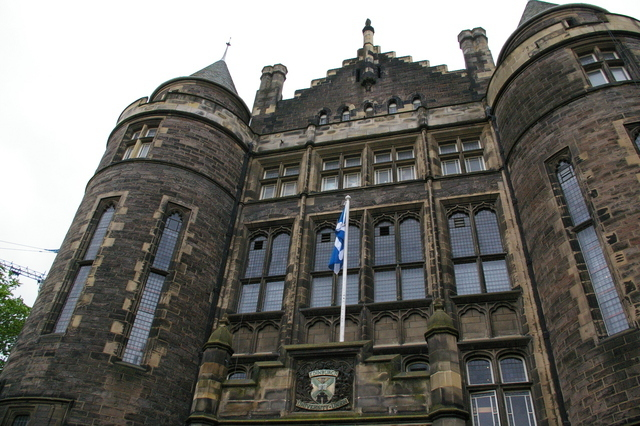
\includegraphics[width=5cm]{image200706/teviot.jpg}
  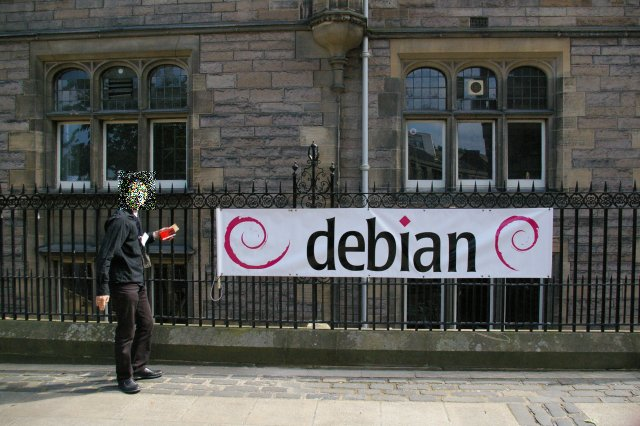
\includegraphics[width=5cm]{image200706/debconf7-debian.jpg}
\end{wrapfigure}
  会場は、エジンバラ大学の建物の一部である Teviot という名前の
  建物を借り切り、開催されました。

 参加者はふたつのホテルに分散して宿泊していたのですが、それらのホテルから歩いて
  10 分ほどのところにあります。
\\

\begin{itemize}
  \item Upper Talk Room: 	メイン用。250人ほど入ることができます。\\
	\begin{minipage}{0.4\hsize}
	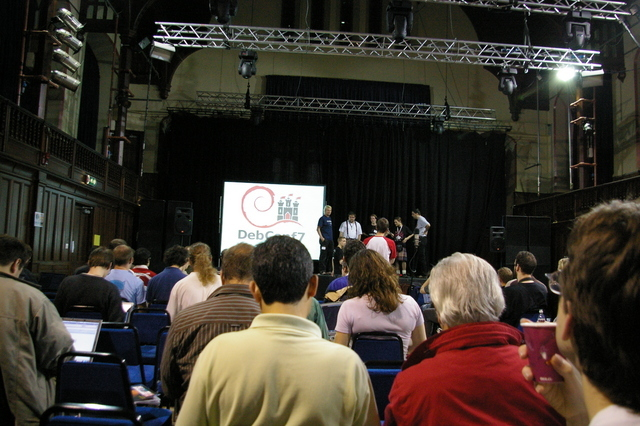
\includegraphics[width=0.8\hsize]{image200706/debconf7-upper-talk.jpg}
	\end{minipage}
  \item Basement Talk Room\\
	サブ用。50人ほど入ることができます。
  \item Lower BoF Room\\
	BOF 用。20人ほど入ることができます。
  \item Upper BoF Room\\
	BOF 用。20人ほど入ることができます。
  \item Hacklab 1: 	ハック用。\\
	\begin{minipage}{0.4\hsize}
	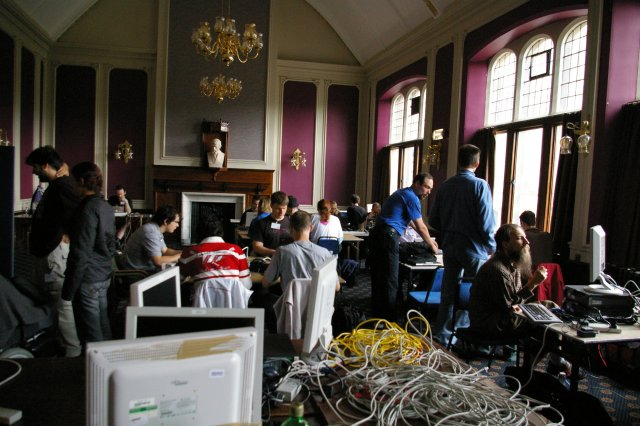
\includegraphics[width=0.8\hsize]{image200706/debconf7-hacklab00.jpg}
	\end{minipage}

  \item Hacklab 2: ハック用。通常はバーらしいです。\\
	\begin{minipage}{0.4\hsize}
	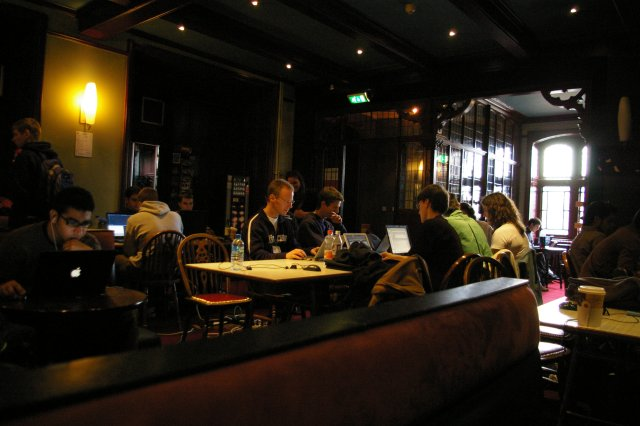
\includegraphics[width=0.8\hsize]{image200706/debconf7-hacklab01.jpg}
	\end{minipage}
  \item Night venue:
	廃墟と化した教会。パイプオルガンがあったりします。
	夜の22時以降は Teviot を使うことができないので
	ここを借りてみんなでハックしたり、話し合ったりしました。
\\
     	\begin{minipage}{0.4\hsize}
     	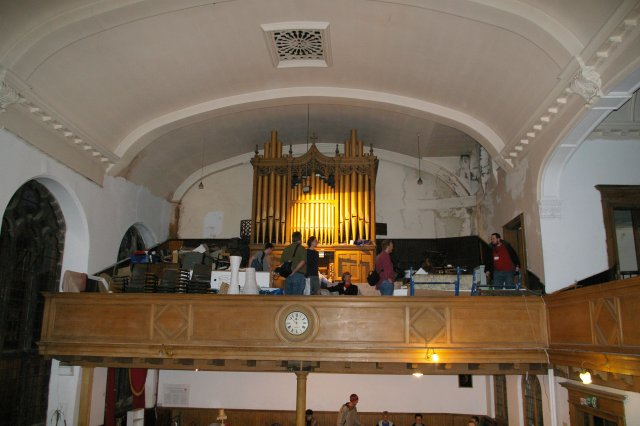
\includegraphics[width=0.8\hsize]{image200706/debconf7-elsewhere.jpg}
     	\end{minipage}
     	\begin{minipage}{0.4\hsize}
     	\end{minipage}
\end{itemize} 

\subsection{スケジュール}

\begin{wrapfigure}{r}{8cm}
 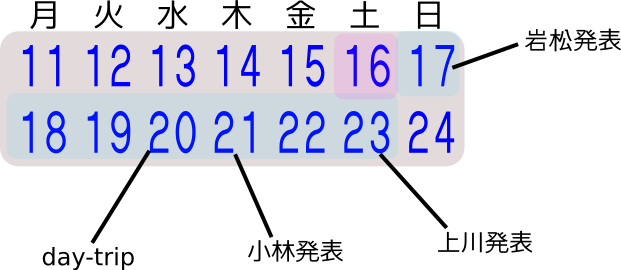
\includegraphics[width=1\hsize]{image200707/schedule.png}
\caption{全体スケジュール}
\label{fig:schedule}
\end{wrapfigure}
16日のDebian Day で Debian Conference は開始し、23日まで毎日いろいろな予
定がくまれていました。
20日だけはカンファレンス参加者で day-trip を実施しました。

\begin{wrapfigure}{r}{8cm}
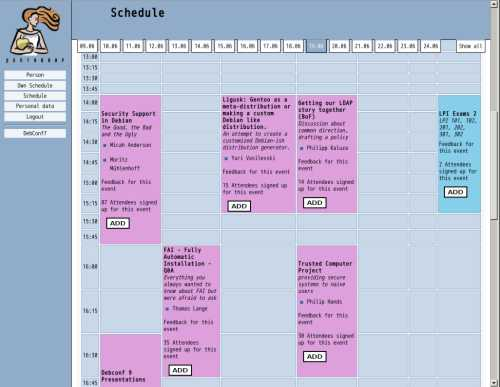
\includegraphics[width=8cm]{image200707/penta.png}
\caption{pentabarf 画面}
\label{fig:penta}
\end{wrapfigure}
 スケジュールは ruby-on-rails で実装された 
pentabarf システム(\fgref{fig:penta})で管理していました。
スケジュールには
随時変更がかかり、IRC bot での通知がなかったら誰も状況においつけなかっ
 たでしょう。


\subsection{主となった討論}

\subsubsection{組込み系についての白熱した議論}

ARM EABI の導入が大きなトピックです。日本から SuperH の
話題ももっていきました。マインドシェアがおおきくなっているようです。
また、組込関係の対応を Debian で行うための議論も行われました。
New DPL の Sam Hocevar が組込み関係に興味があるようなので、
いままで停滞していた組込み関係による成果のマージが加速するかもしれません。

\subsubsection{バージョン管理システムとソースコード管理の話}

git の利用方法のチュートリアルや、arch を例にとってのDebianディストリビュー
ションのフォークをメンテナンスするためのソースコード管理のやりかたについ
ての紹介がありました。git などの普及により分散SCMが普及し、ソースコード
の管理のワークフローに影響しており、再考が必要だという風潮が見られました。

特に ubuntu でソースコード管理を見直しており、bazaarを中心としてブランチ
をdpatchのパッチファイルに変換したりするツールなどのインフラがととのい始
めているということが大きいようです。

\subsubsection{翻訳についての議論}

翻訳関係の話が毎日行われました。毎日議論を重ね、議論した結果を毎晩ドキュメント
を修正していました。
また、時期リリースの lenny までに、翻訳のインフラやドキュメント整理
を行う予定だそうです。

小林さんの翻訳関係のインフラに関するセッションがあったのですが、
小林さんが来られなかったので、上川さんが代理で BOF を行いました。
各国で使用されているツールの紹介などがありました。日本でも導入を検討
をする必要がありそうです。

\subsubsection{Daytrip}


\begin{wrapfigure}{r}{5cm}
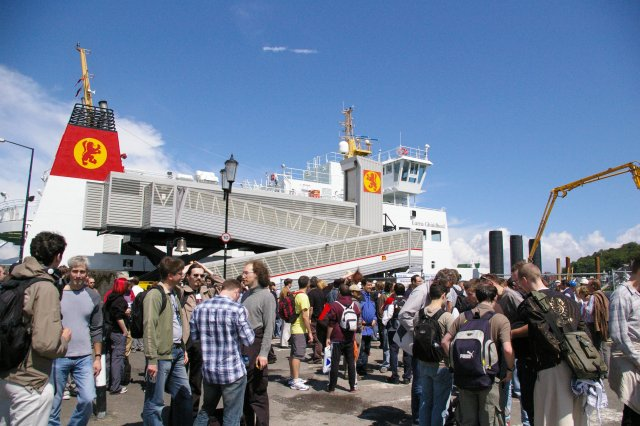
\includegraphics[width=5cm]{image200706/debconf7-daytrip.jpg}
\end{wrapfigure}

Debconf では一日、参加者で旅行をするというイベントがあります。今回の
Debconfでは Rotheway (Bute島) でまったりとピクニックをしました。Rotheway 
への移動は、Edinburgh から Glasgow へ電車で移動し、Glasgow からさらに電
車で Wemyss Bay へ移動します。Wemyss Bay は Rotheway 行き専用の舟着き場
で、そこから船に乗って Rotheway に移動しました。

Rotheway の町は島で、特になにもないところです。ほとんどの建物は売出中で、
裁判所の建物も売りに出ていました。財政がやばそうな感じです。
建造物としては、教会や、バイキングの侵略の際に戦った城がありましたが、修復中でしかも工事は止まっていました。
山の奥へ1時間ほど歩くと、湖があり、大抵の参加者はその湖でピクニックをしたり、ボード
に乗って遊んでいたようです。

\debconfsection{Debconf 2007 各種討議内容}{岩松 信洋、矢吹 幸治、上川 純一}
\label{sec:debconf2007detail}
\index{Debconf2007}
\index{Debconf}

2007年度の Debconf は 6月13日から6月23日まで、スコットランド、エジンバ
ラで開催されました。2007年度の Debconf の討議内容を以下にまとめます。

\subsection{6月16日の発表内容}
\subsubsection{simple-CDD}

CDD を簡単に準備できる仕組み。reprepro を使ってミラーを作成している。
debpartial などはうまくうごかないことが多かったらしい。会場からはなぜ
aptitude とかを利用しないのかという質問は出ましたが、そこまで検討してい
ない、とのことでした。

\texttt{--qemu} オプションを指定したらイメージを作成して qemu でテストす
るところまでしてくれるそうです。\texttt{build-simple-cdd} コマンドを使えば簡単に
CDDがつくれるそうです。

\subsubsection{64studio}
Debian ベースの音楽関係のソフトウェアを収録したCDD(Common Debian
Distribution)です。各音源を組み合わせて、音を組み上げていくJackというプ
ログラムの説明などをしていました。イコライザーとしてJaminを利用し、出力
の周波数特性をフリーハンドで変えることができるデモをしていました。また、
PCのキーボードをつかって、パイプオルガンシミュレータ aeolus の(鍵盤の)キー
ボードを使って演奏するデモもしていました。

\subsection{6月17日の発表内容}
\subsubsection{Welcome talk}
  開会の挨拶。スポンサーと開催にかかわってくれた人たちへの感謝のコメントを
  行いました。非常にシンプルに終わった開会式でした。
	
\subsubsection{About porting SuperH for Debian}
  Renesas 社製 CPU SuperH の Debian へのポーティングの話でした。SuperH を 
  Debian にポーティングしている途中経過と現在発生している問題、および今後
  の課題について話し合いました。組込み関係の人が参加してくれていたが、みな 
  ARM にかかわっているので直接の支援は難しそうな印象をうけました。

\subsection{6月18日の発表内容}

\subsubsection{bugs.debian.org and debbugs}

BTS の開発についての進捗報告でした。いろいろな機能が追加されているのです
が、歴史的経緯でdone状態の遷移とバージョントラッキングで問題が解決してい
るかどうかという状態の遷移に整合性がとれないようになっているという話題が
でました。この部分については互換性をなくしてでも解決してよいのではないか、
という討論をしました。また、SOAPインタフェースの新しい機能の紹介などもあ
りました。

\subsubsection{Embedded Debian}

  Debian の組込み向けプロジェクト Emdebian の話です。今まで行ってきた方
  法の説明と結果を報告し、今後の方向性について話しをしました。 現在の 
  ftp-master 達はクロスビルドは受け付けてくれません。この問題を解決する
  ためにパッケージにタグを付けたりして対策する予定とのことです。
  Embedded 用のツールも用意しており、これらを使ってクロスビルドできるよ
  うになりました。 しかし、全てのパッケージはチェックできず
  \begin{commandline}
  make check
  \end{commandline}
  や
  \begin{commandline}
  make nodocs
  make nocheck
  \end{commandline}
  を使うように修正する必要があることを提案しました。
  その他の問題は後日行われた BOF で議論されました。

\subsubsection{Debian Live}
 Debianのサブプロジェクトとして活動しています。ツールは Ubuntu の casper 
 からforkして作成したものです。国際化も国コードやキーボードを入れるよう
 にするみたいです。自分で会社を興して、キオスクシステムのために開発をし
 たとのこと。また、usb ブートなどもサポートしているので、コンピュータ本
 体に情報が残らなく、銀行などからも引合があると話していた。こちらから
 i18nに関連した質問をしたら、日本の市場に興味があるようで、あとで、すで
 に作ってあった日本用のCD イメージを見せてくれました。

 \url{http://download.webconverger.com/i18n/jp/webc-2.21.jp.iso} からダウンロー
 ドできます。

\subsubsection{Debian Armel Port}

Armel の Debian へのポーティングの話でした。

\subsubsection{OpenStreetMap}
  Free な地図をつくるためのプロジェクトの話です。Google Map がすでに存在し
  ていますが、DFSG-Free ではないので、GPS 等を使って、自由に扱える地図を
  つくるということが目的です。ライセンスは Creative Commons を採用しています。

  \url{http://www.openstreetmap.org}

\subsubsection{Wacky Ideas II}
  Wacky Ideas というのは、こんな凄いこと考え付いちゃったぜというのを、ディ
  スカッションしてまともなものにしていく、ブレーンストーミング系のセッショ
  ンです。

  口火をきったのは、 Ian Jackson による upstream, ディストリビューション, 
  派生ディストリビューションで無駄なことしてないか? これらを包括するよう
  なVCS(Version Control System)って作れないか? って話。

  次は、Ubuntu の言語パックのように、翻訳 debを作るべきかと言う話題でし
  た。この方法は翻訳の部分が小さいのであればオーバヘッドが大きすぎる。そ
  のためパッケージをまとめて扱うことになるだろうとうことでした。極端なや
  り方として Ubuntu は、(1つで) 100MB のパッケージとして対処しているとい
  うことです。

\subsection{6月19日の発表内容}
\subsubsection{Debian virtualization support}
  Debian での仮想化ツールサポートの話です。あらゆる仮想化のシステムをサポートし、
  それらをサポートするための独自のツールを開発していることを紹介しました。
  また、仮想化ツールを使った、Debian パッケージのメンテナンスの話をし、
  ユーザー側だけでなく、開発者側から使い易くするために行っている活動をアピール
  していました。

\subsubsection{From Concept to Concrete}
  ハードウェアの企画、提案、そしてできるまでを、 Daniel Silverstone と 
  Vincent Sanders がコント風で行っていました。自分たちのハードウェア設計
  会社の紹介をしたかっただけなのかもしれないです。

\subsubsection{PC Install and Backup Management}
  発表者が来れなかったので、集まったみんなでディスカッションして進めるこ
  とになりました。まず、みんなどんなツールを使っているかと言う話題になり
  ました。

  unstableに、boxbackupというソフトウェアがあるから使っているいう人から、
  mondo, rsync, cpio, tar などを使っている人もいました。また、サーバ上でシステ
  ムをバックアップするために lvm-snapshot を使わないといけないんだという人
  は、Mysqlのデータベースの同期機能を利用していました。

  つぎに話題は、d-i (Debian Installer) を使って、大量にインストールする話
  題になりました。preeditを使って同じようにインストールする手法や、FAIを使う方
  法などがでてきました。


\subsubsection{Debconf 9 Presentations}
  Debconf 9 のプレゼンテーションです。
  Debconf 8 は アルゼンチンに決定していますが、
  Debconf 9 はまだ未定です。このセッションでは、Debconf 9 の立候補地域による
  プレゼンテーションを行いました。
  現在のところ、立候補地はスペインの Extremadura のみです。
  食事施設や宿泊施設が充実しており、プールもあるとのことです。
  この流れだと Debconf9 は Extremadura に決まりそうです。
  詳細は \url{http://wiki.debconf.org/wiki/Extremadura} からみることができます。

\subsubsection{Emdebian BOF}

  Debian の組込向けプロジェクトである Emdebian の BOF でした。uClibc の
  サポートおよび、busybox をベースにしたユーザーランドのサポートについて
  議論しました。既にサポートの体制を整えるようにしているが、uClibc をサ
  ポートしてしまうと、uClibc 用のバイナリを作成する必要があるので、バイ
  ナリの数が倍になってしまいます。この問題をどのように解決していくか、今
  後議論を重ねていくとのことです。

  Busybox の話は、busybox をベースにした場合、動くパッケージと動かないパッケージが
  出てしまいます。これは busybox をベースとして使用しているため発生する問題です。
  組込みでは busybox の base system を考える必要があるので、現在どのパッケージが動かない
  のかを調査している段階です。調査した結果は wiki にまとめられています。
  \url{http://wiki.debian.org/EmdebianRootfs}

\subsubsection{Keysigning Party}

今年は、キーサインに集まった人達を4つのグループに分けて、各グループを大
きめの部屋で分割してキーサインを行いました。全員がキーサインをするには巨大な
場所が必要だったので分割したのでしょう。

キーサインには finterprint を印刷した紙が必要です。そこに計算したsha1の
結果を書き込んで持参するのですが、その値
(sha1sum出力)が読み上げられ、同じ結果が出たことが確認できた人だけが書名
できます。

各人は国家の発行する公的な写真つきの証明書(例えばパスポート)を見せ、
fingerprint, sha1の計算結果について確認していきます。

分割したおかげか今年は30分程度で終わりました。

\subsection{6月20日の発表内容}
\subsubsection{Daytrip}

Debconf では一日、参加者で旅行をするというイベントがあります。今回の
Debconfでは Rotheway (Bute島) でまったりとピクニックをしました。Rotheway 
への移動は、Edinburgh から Glasgow へ電車で移動し、Glasgow からさらに電
車で Wemyss Bay へ移動します。Wemyss Bay は Rotheway 行き専用の舟着き場
で、そこから船に乗って Rotheway に移動しました。

\begin{wrapfigure}{r}{5cm}
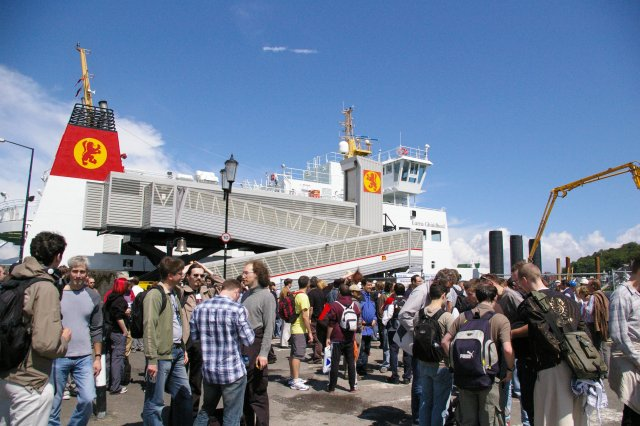
\includegraphics[width=5cm]{image200706/debconf7-daytrip.jpg}
\end{wrapfigure}

Rotheway の町は島で、特になにもないところです。ほとんどの建物は売出中で、
裁判所の建物も売りに出ていました。財政がやばそうな感じです。
建造物としては、教会や、バイキングの侵略の際に戦った城がありましたが、修復中でしかも工事は止まっていました。
山の奥へ1時間ほど歩くと、湖があり、大抵の参加者はその湖でピクニックをしたり、ボード
に乗って遊んでいたようです。

\subsection{6月21日の発表内容}
\subsubsection{Forking Debian every day}

GNU arch でいかに SELINUX版のDebianのポーティングを楽にしたか、というワー
クフロー紹介のセッションのはずでしたが、いろいろと技術的な障害があったよ
うで、 git でDebianのパッケージをメンテナンスするための方法をデモンスト
レーションするセッションに急遽変更されました。アプリケーションの各種機能
をSCMのブランチの機能を利用して実装し、新しいバージョンがリリースされて
もSCMの機能が活用できる、という話題でした。

\subsubsection{Quality assurance activities for localization}

小林さんが提案を提出し通っていたのですが、なぜか Debconf7 に参加しなかっ
たのと、報告・周知・対策を何も講じなかったため開催されるはめになりました。

急遽 IRC で現地と日本を結んで上川がセッションを行いました。フランス、ブ
ラジルなどのチームでの翻訳の進め方やツールの使い方についてディスカッショ
ンを行いました。メーリングリストをスキャンしてくれるロボットツールがあ
り、日本翻訳チーム向けに使えるように調整してくれるとのことでした。

\subsubsection{Debian ceilidh/Sun Drinks Reception}
\begin{wrapfigure}{r}{5cm}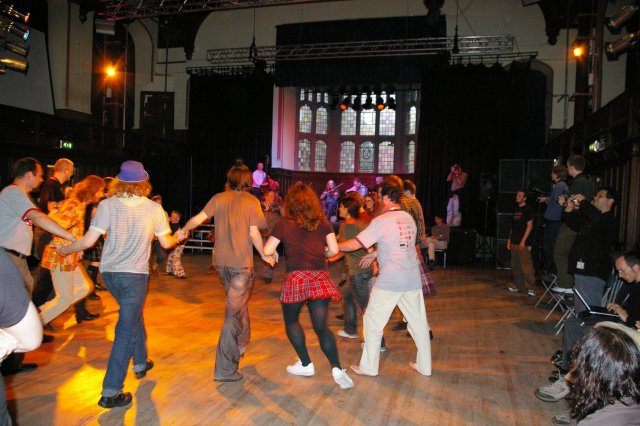
\includegraphics[width=5cm]{image200706/debconf7-dance.jpg}\end{wrapfigure}

Sun Microsystems と Google のスポンサによるパーティでした。Sun が飲み物、
Google がピザを提供してくれました。また、スコットランドの民謡の演奏家を呼
び、大ホールに集まったパーティ参加者達でスコットランドのダンスを楽しみま
した。

\subsection{6月22日の発表内容}

\subsubsection{Derivatives Round Tables --- Debianより派生したディストリビューション}

Benjamin ``Mako'' Hill が司会を務める、Debian より派生したディストリビュー
ションの関係者が集まってのパネルセッションでした。ベネズエラで開発されて
いる国の支援を受けたディストリビューション、スペインの Extremadura、
Debian Edu, Ubuntuなどが参加してきていました。予想どおり白熱しました。ディ
ストリビューションからのフィードバックの部分が問題になっていました。BTS 
の共有などもトピックになっていました。

\subsubsection{Proactive Bug Discovery}

  DPLである、Sam Hocevar のセッションでした。
\footnote{このセッションの英語は矢吹にはわかりやす
  かった。}ソースを全部チェックするのは非常にコストが高いので、クリティカ
  ルな部分だけは全部査読するが、ほとんどの部分は、ツールを使って機械的に
  チェックするだけもかなりのことがわかるとのことでした。

ソースコードを正規表現でスキャンしたり、google のコードサーチエンジンで
  チェックしたり、コンパイラーにチェックさせたりという部分について語って
  くれました。

\subsection{6月23日の発表内容}

\subsubsection{debian-community.org}

  Debianコミュニティに対する問題意識から、
  \url{http://debian-community.org} の提案セッションが行われました。
  Ubuntuコミュニティの事例からとったものです。Debian開発者になり活躍する
  までの時間がかかるのが問題意識となっています。その問題を解決するべく、
  debian-community.orgというサイトを作り、Debianコミュニティ活動すると宣
  言し、活動している間はメールの転送などのサービスを提供します。活動が一定
  期間止まったら、この活動リストより外されます。他にもplanetや、wikiなどの
  提供を行う予定があります。

  問題点としては、これまでのローカルコミュニティとの整合性、debian.org 本
  体もコミュニティであること、新しいコミュニティを作ってドライブしていく
  だけの魅力がそこにあるかなどが話し合われました。

\subsubsection{WTFM, again: Write The Fine Manual page}

Debian package で頒布されているプログラムには man が付属していないと
いけないということが Debian Policy で決まっているが、nroff 形式の man
は時代遅れです。man だけでなく、あらゆるフォーマットに対応したドキュメントを
容易に作成するにはどうしたいいのか話し、DocBook XML を使った場合の簡単な
チュートリアルを行いました。
また、man はあるが、Linux の man ではく、Unix の man だったりすることが
あるので、ユーザーに man を提供する際に注意すべき事などを話しました。

Debian package で頒布されているプログラムには man が付属していないといけ
ないということが Debian Policy で決まっているが、norff 形式の man は時代
遅れです。man だけでなく、あらゆるフォーマットに対応したドキュメントを容
易に作成するにはどうしたいいのか話し、DocBook XML を使った場合の簡単な
チュートリアルを行いました。また、man はあるが、Linux の man ではく、
Unix の man だったりすることがあるので、ユーザーに man を提供する際に書
いてある内容が本当に妥当なのか確認すべき事などを話しました。
 
\subsubsection{pbuilder talk}

上川 純一 がpbuilder, cowbuilder, qemubuilder についての議論を行いました。
pbuilder を利用しているユーザは非常に多いが、qemubuilder の利用者は数人
もいなかったということがわかりました。また、マニュアルの存在をしらない 
人が多数いました。

\subsubsection{Lightning Talks}

ライトニングトークは若干オーガナイズに失敗しており、最初計画していたメン
バーがあまりいなかったため、好きな人が好きなことを語るという会になってし
まいました。

\subsubsection{Closing ceremony}

最後のしめの挨拶がなされ、スポンサーに感謝したりしました。

\subsection{講演以外のできごと}

\subsubsection{apt-listbugs 関連の討論}

Don Armstrong がきており、bugs.debian.org の SOAPインタフェースを拡張し
た、といいました。apt-listbugs の実装を変更し、SOAPインタフェースを利用
するようにし、現在サーバ側で生成しているインデックスファイルが、もう必要
ないようにしました。現地で SOAP インタフェースのデバッグを実施し、実用に
なるようにしました。

また、 debian-changelog-mode に以前パッチをおくってくれた Luca Capello 
と BTS の HTML をパースしているからださいんだよ、という話をしたら、 SOAP 
を emacs からつかうのはいやなので、apt-listbugs を使おうという話になり、 
apt-listbugs list コマンドを拡張して実装することになりました。しかし、そ
れが実装されるまえに、vim のメンテナ Stefano Zacchioli がその話をうしろ
で聞いていて、その場でvim 用の debian/changelog での closes: 補完コードが
実装されてしまいました。

\subsubsection{QEMU 関連の討論}

上川は qemu、qemubuilder 関連で熱く議論してまわりました。

Thiemo Seufer (QEMU mips ポートのメンテナで QEMU のコミッタ、および
Debian の MIPS ポートのメンテナ)と議論しました。chroot 内部での qemu
user emulation をいかに static link をしないで実施するのか、という点につ
いて議論し、環境変数を定義する必要があるね、ということで合意しました。

夕食の時間で Ottavio と議論し、qemubuilder の設計と、qemu system
emulation ではなく qemu user emulation での実装について議論しました。


\subsubsection{矢吹×grisu}

aptにi18n機能がマージされたのにまだサーバ側のインフラの整備が行われていま
せん。矢吹はDDTPの担当者の Grisu と DDTP の展開について議論しているようで
した。なんらかの成果がでるとよいですね。

\subsection{来年の Debconf}

来年の Debconf はアルゼンチンで8月に行われます。日本は夏ですが、アルゼン
チンは冬です。冬期合宿になると思いますので、気合いをいれていかないと、ひ
どいことになるかもしれません。気を付けましょう。

\dancersection{OSC-Kansai 参加報告}{山下 尊也}
\label{sec:osckansai2007}
\index{Open Source Conference@Open Source Conference}
\index{かんさいでびあん@関西Debian勉強会}
\index{debianjp@Debian JP}

\subsection{開催概要}
関西 Debian 勉強会は、7月20,21日に京都コンピュータ学院で開催されたオープ
ンソースカンファレンス2007 Kansai(以下、OSC Kansai) に 京都ならびに関
西地方でも Debian のプレゼンスを向上させるため参加しました。
また、7月の関西Debian 勉強会としての位置
付けで、第4回 関西Debian 勉強会としています。

1日目は、背広族の方が多いと思っていましたが、そこまで多くなく、京都コンピュー
タ学院の生徒さんが多かったです。

2日目は、関西 Debian 勉強会からブースへの協力して頂いた方が多かっ
たので、入口の真っ正面である京都コンピュータ学院のシンボルでもある階段の
下にブースを移動し、さらに多くの方がブースに足を運んでいただきました。

\begin{figure}[H]
 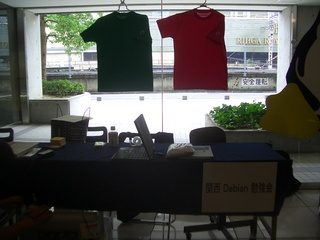
\includegraphics[width=0.5\hsize]{image200708/0720booth.jpg}
 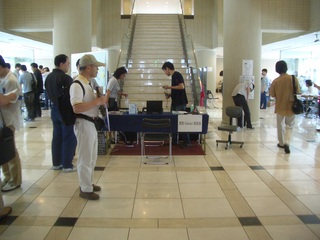
\includegraphics[width=0.5\hsize]{image200708/0721booth.jpg}
\caption{展示風景}
\label{fig:osctenjifukei}
\end{figure}

\subsection{セッション}

今回、セッションは13:00-13:45と言う45分間しかありませんでしたが、25人の
方に参加して頂きました。以下の内容について行いました。

\begin{enumerate}
 \item 関西 Debian 勉強会とは 山下 尊也
 \item Debian.org / Debian JP / 関西 Debian 勉強会の関係 矢吹 幸治
 \item Debconf 7 ミニ報告 + Debconf 日本開催について。 矢吹 幸治
\end{enumerate}

講師は、DebianJP会員であり、関西 Debian 勉強会について動いている私と矢吹さん
が行いました。

私のセッションは、関西 Debian 勉強会とはという題で、OSC Kansaiに参加して
頂いてる方にも、関西 Debian 勉強会に今後参加して頂けるように、参加し易い
勉強会をアピールしたかったので、いくつかの笑いを入れて説明しました。
第3回での「ブルースマン」さんのファイアーウォールフリーダムの画像や、なぜ、
関西 Debian 勉強会のシンボルが「ほっけ」であるのかを説明すると、会場から
は笑いが起こりました。

矢吹さんのセッションは、今まで、Debian JPと関西 Debian 勉強会との関係に
ついて述べる機会がなかったので、参加して頂いた方には、関係などが理解して
頂けました。具体的には、8月12日(日)に神戸研究学園都市で行われた第5回
関西 Debian 勉強会で、参加費について議論した際に、OSC Kansaiで聴いていた
ため、分かり易かったとおっしゃって頂きました。ただ、今まで関西 Debian 勉
強会では、このような関係について述べる機会が少なかったため、今後機会を増
やす必要があると思いました。
また、Debconfについては、矢吹さんの Debconf で手に入れたお土産を景品にし
て、クイズを行いました。クイズ形式でしたが、手をあげて頂ける方が少なかっ
たのが残念でした。関西国際空港もありますので、関西で開催出来そうな
場所を教えていただけるように働きかけました。

\subsection{ブース企画}

\subsubsection{リアル掲示板}

今回、関西 Debian 勉強会では、みなさんの意見を付箋紙に書いてもらい、
Debian についての意見を書いてもらいました。

\begin{figure}[H]
\begin{center}
  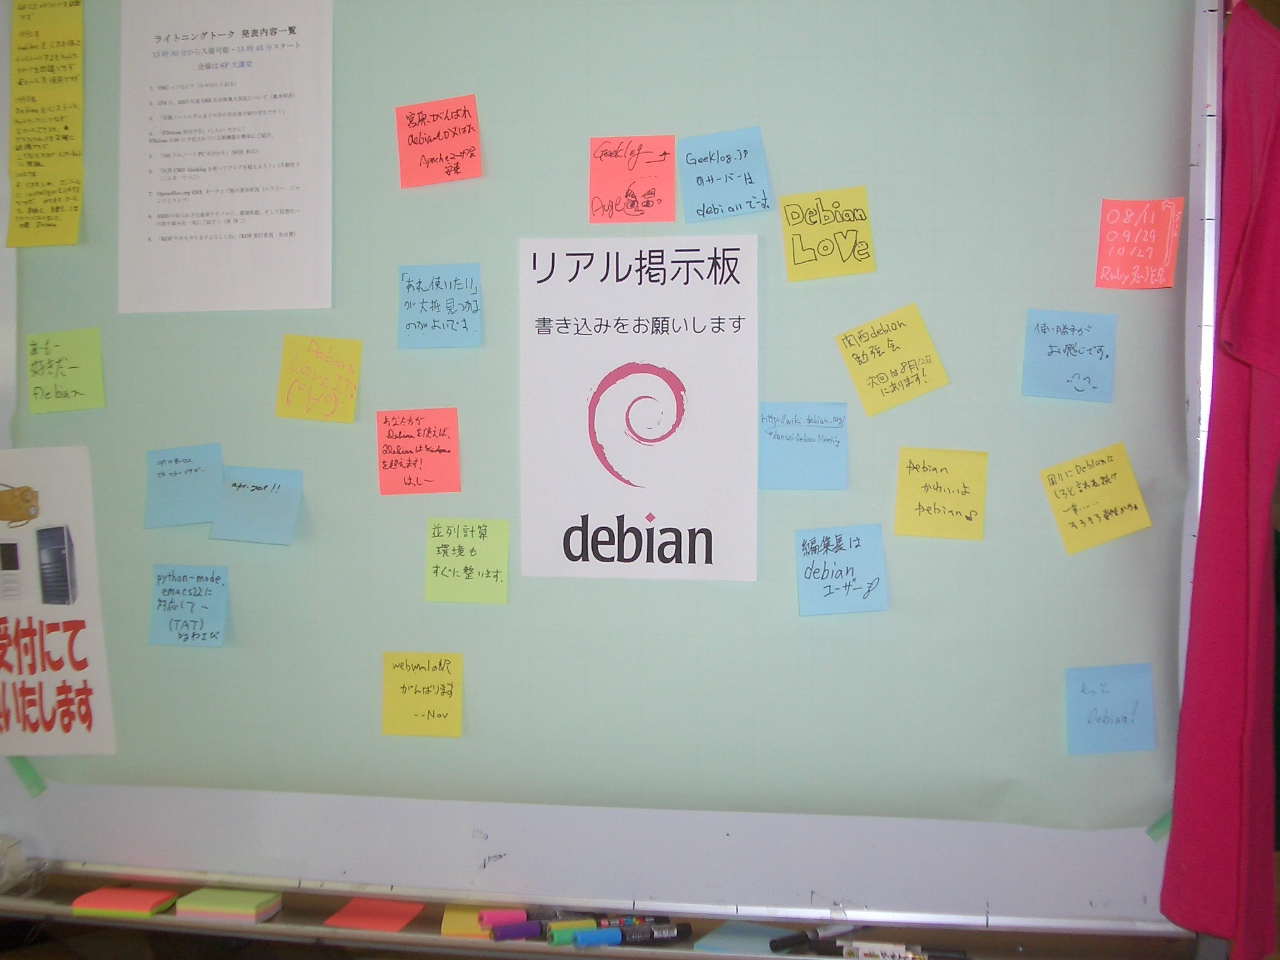
\includegraphics[width=\hsize]{image200708/real-keijiban.jpg}
\end{center}
\caption{リアル掲示板}
\label{fig:realkeiji}
\end{figure}

集まった意見は下記です。

\begin{multicols}{2}
 \begin{itemize}
 \item Debian Love IT! \verb|(・∀・)|
 \item 宮原がんばれ debian もがんばれ Apache ユーザ会 安東
 \item 「あれ使いたい」が大抵見つかるのがよいです
 \item Geeklog.JP のサーバは debian でーす。
 \item Debian Love
 \item lilo.linux.or.jp も Debian で動いています by ohura
 \item Sumibi.org も Debian で動いています! by kiyoka
 \item 編集長は Debian ユーザ!
 \item もっと Debian!
 \item Debian かわいいよ Debian ♪
 \item 使い勝手がよい感じです。
 \item 周りに Debian にしろと言われ続け一年…そろそろ覚悟かなぁ
 \item aptは使いますよ。でもマカーですが…
 \item apt-get !!
 \item python-mode emacs22 に対応してー \verb|(TAT)| by わさび
 \item webwmlの訳がんばります --Nov
 \item 並列計算環境もすぐに整います。
 \item あなた方が Debian を使えば、DebianはWindowsを越えます! はっしー
 \item あーもー好きだー Debian
 \item 1998年 Debian をインストール、ネットワークに繋ぎ、Eメールできるも、
       グラフィックカードを正確に認識できず、LYNXのみでインターネットに
       接続。
 \item 2007年 今、CDを入れ、コンソールに installguit と入力するだけで、WEBもメー
       ルも、動画も、音楽も、しほうだいになりました。万歳 Debian
 \end{itemize}
\end{multicols}

サーバでもデスクトップでも、本当にみなさん、Debian を愛してますね
\verb|:)|

個人的に気になったのは、python-modeについてですが、Emacs22から
python-modeは付属する形に変更されたみたいで、私のsid 上のEmacs22では
python-modeが動いています。

\subsubsection{配布・販売物}

以下のものを配布しました。

\begin{itemize}
 \item フライヤー
 \item DVD
\end{itemize}

\begin{center}
 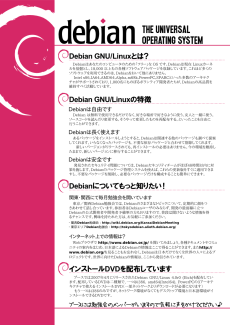
\includegraphics{image200708/flyer.png}
 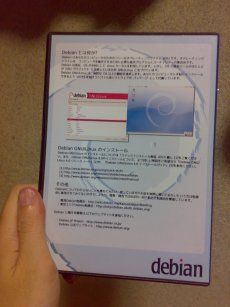
\includegraphics{image200708/dvd.jpg} 
\end{center}

関西 Debian 勉強会では、OSC Kansai で配布を行うために、矢吹さんが提案し
て頂いたフライヤーを参考に、日本人向けに作り替えるために、のがたさんがデザイン
を担当し、かがさん、倉敷さんなどが文章を考えました。

また、DVDジャケットについても、かがさんがデザインを担当し、武藤さんのイ
ンストールガイドのURLが書いてあったり、ジャケットが格好よかったので、家
に飾りますとおっしゃられた方もいらしゃいました。ただ、より多くの方に
Debian について知ってもらうために、Debian を使っていらっしゃる方
には周りの人に配布して下さいとお願いしました。

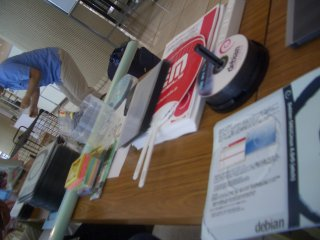
\includegraphics{image200708/booth2.jpg}
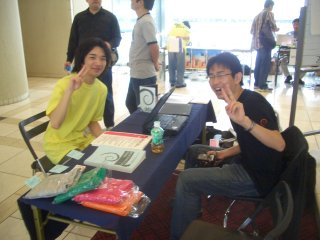
\includegraphics{image200708/booth.jpg}

以下のものを販売しました。

\begin{itemize}
 \item Tシャツ
 \item ステッカー
 \item 「あんどきゅめんてっど でびあん」2006年冬号の冊子
\end{itemize}

料金については、今年の3月に行われた OSC Spring と一緒にし、Tシャツとシー
ルは小室さん、「あんどきゅめんてっど でびあん」の冊子は岩松さんに私の家
に送って頂き、委託販売と言う形で行いました。
背景として、私が関西 Debian 勉強会に Debian Tシャツを着ていくと、やはりグッズが
欲しいなぁと言っていただいたり、紙媒体で情報が欲しいって方がいらっしゃっ
たので、実現しました。

当初、僕が予想していたものよりも多くの売り上げがあり、やはり冊子でみたい
と言う意見や、Tシャツの黒色が欲しい、Mサイズが欲しいなどの意見もありまし
たので、11月9,10日に大阪南港ATCで行われる関西オープンソースフォーラムで
もグッズの販売を行いたいと思います。

売り上げですが、Tシャツ(1枚2000円)が11枚。冊子(1部1000円)が7部。ステッ
カー(1枚300円)が12枚で、合計32,600
円(2000円*11枚+1000円*7部+300円*12枚)でした。ご協力頂いた方、本当にありがとうございました。

\dancersection{将来の Debconf }{上川 純一}
\label{sec:debconfplanning}
\index{Debconf}


Debconf は来年はアルゼンチンですが、将来的には日本でも開催できるとよいで
すね。
また、Debconfの開催内容をいかに有益に使えるか、考えてみましょう。


\subsection{成果の活用}

Debian Conferenceには複数の側面があります。成果はどうやってできるのでしょ
うか。

\begin{table}[H]
\caption{参加の成果}
\label{tab:framework}
\begin{center}
{\LARGE
  \begin{tabularx}{\hsize}{|c|X|X|}
 \hline
 & 参加した場合 & 参加しなかった場合 \\
 \hline
 コード	& 合宿してコードがかける &  \\
 \hline
 文書化	& 合宿して文書がかける&  \\
 \hline
 議論 	& 直接議論できる &  \\
 \hline
 発表 	& セッションに参加して発表でき、発表をきくことができる。 &  \\
 \hline
&&\\
 \hline
&&\\
 \hline
 \end{tabularx}
}
\end{center} 
\end{table}

これを踏まえると、開催自体は重要ですが、参加にはおよびません。
あなたも参加したくなってきたのではないですか?

\subsection{日本開催}

Debian Developer の中では Debian Conference を日本で開催したいと思ってい
るメンバーがいます。日本で開催するとすれば、日本で開催するためのチームが
必要です。日本で数度イベントを運営して円滑にすすめられるようにしておくこ
とも必要でしょう。

日本でのDebconfの検討の進捗については
\url{http://wiki.debian.org/DebConfInJapan}
で整理されています。

\begin{table}[H]
\caption{2005年に実施した各種空港に到着するまでのコスト評価例}
\label{tab:framework}
\begin{center}
{\LARGE
  \begin{tabularx}{\hsize}{|c|X|X|X|}
 \hline
 & フランス & アメリカ & 南米 \\
 \hline
成田 & 828 & 809 & 1600 \\
千歳 &980 & 1197 &2121 \\
関西 &736 & 809 &1718 \\
沖縄 &1485 & 1197 &4307 \\
 \hline
 \end{tabularx}
}
\end{center} 
\end{table}

\dancersection{cdn.debian.or.jpの紹介}{荒木 靖宏 (yasu@debian.or.jp, ar@debian.org)}
\label{sec:cdndebianorjp}
\index{debianjp@Debian JP}
\index{cdn.debian.or.jp}
\index{Content Delivery Network}

\subsection{CDNとは}

Content Delivery Network(CDN)はウェブコンテンツ配置および配送方法として
Akamai\index{Akamai} 社によりサービスされ広く知られることになった。当初か
ら一部の人気の高いサーバへのトラフィック集中によるサーバ停止の回避、海外
のリッチコンテンツ取得の高速化、トラフィック分散によるネットワークおよび
サーバの利用平準化などの理由で広く受け入れられた。

CDNという用語自体はWWWに限ることなく、一般にコンテンツを取得するための配
送手段や方法全体を指す場合がある。たとえば、Winny\index{Winny} や
Bittorrent\index{Bittorrent}などのコンテンツを取得するために特別に設計さ
れたプロトコルを用いて、P2Pネットワークを構成するような手法も含まれる。

\subsection{DebianにおけるCDNの現状}
\subsubsection{利用法とユーザから見た動作}

\url{cdn.debian.or.jp}ではDebianでインストール時から広くdebファイルの入手に使
われるaptで使えるCDNとして設計し、運用している。そのため、Debianにおける
CDNの利用法は至極簡単である。\url{/etc/apt/source.list} に記述するAPT リポジト
リとして、

\begin{commandline}
 deb http://cdn.debian.or.jp/debian/ stable main contrib non-free
 deb-src http://cdn.debian.or.jp/debian/ stable main contrib non-free
\end{commandline}

以上のように指定するだけでユーザは今までとなんら変わることなくaptコマンド
を使用できる。サービス時の手順と構成は以下のようになる。
(\fgref{fig:usercdndebianorjp})

\begin{enumerate}
 \item  ユーザがapt-get コマンドを行うとcdn.debian.or.jpをDNSで問い合わせる
 \item  \url{cdn.debian.or.jp}を管理するDNSはサーバ候補(surrogate)選択する
 \item  選択結果をDNSのリプライとして返す
 \item  aptは\url{cdn.debian.or.jp}としてSurrogate Cを使用する
\end{enumerate}

\begin{figure}[H]
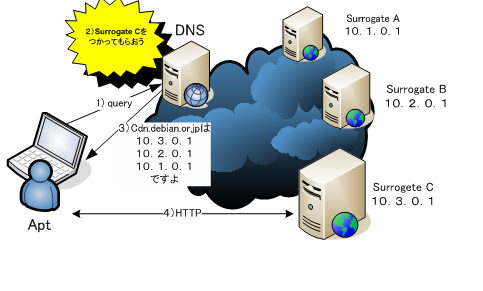
\includegraphics[width=\hsize]{image200708/surrogate.png}

 \caption{ユーザから見たcdn.debian.or.jpの動作}
 \label{fig:usercdndebianorjp}
\end{figure}

\subsubsection{cdn.debian.or.jpのシステムと動作}
CDNシステムが完全に動作しユーザから使用されるためには、システムが完全な
ファイルを提供すること、システムが安定して動作すること、そしてCDNを使っ
た場合に高速に動作していることが求められる。

\subsubsubsection{提供ファイルの完全性}

このために以下二点を満たさねばならない。
\begin{itemize}
 \item  個々のファイルがコンテンツ提供者たるdebファイル配布元と同一であること
 \item  apt-get updateの結果取得するファイル群がどのSurrogateでも入手できること
\end{itemize}
前者については、debはそのファイルのmd5値、sha1値とともに配布され、ユーザ
が使用するaptで確認後に利用されるためCDNを使用した場合でも問題にならない。

後者についてはユーザがapt-get updateを行ったときに接続するSurrogateと
apt-get dist-upgradeを行ったときに接続するSurrogateは同一であるとは限らな
いため、DNSがSurrogateとして返すサーバが保持するファイルは同一である必要
がある。\url{cdn.debian.or.jp}ではDebianプロジェクトで一般に行われている
方法と同様に、rsyncプロトコルを用い、pushミラーを行っている(図2)。その
ため、\url{cdn.debian.or.jp}のサロゲート内で最上流にあるサーバとミラーが
同一であることを2分毎にrsyncミラー終了時に作成されるスタンプファイルを確
認して、同一でないサーバはサロゲート候補から一時的に除外している。

\begin{figure}[H]
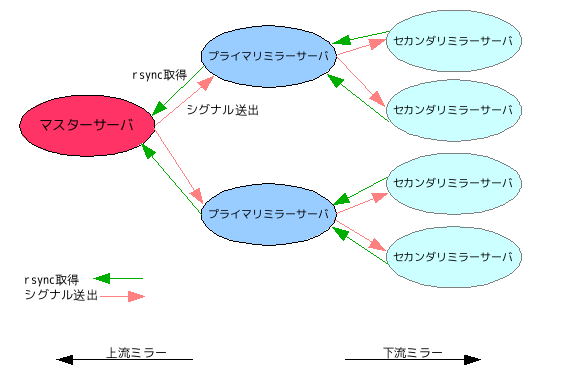
\includegraphics[width=\hsize]{image200708/pushmirror.png}
 \caption{Debianサロゲートのrsyncによるミラー}
 \label{fig:rsyncsurrogatemirror}
\end{figure}

\subsubsubsection{システムの安定動作}
先に述べたように、ユーザはCDNを使用する際にはDNSを最初に使用するため、
DNSの安定運用がカギとなる。そのため、\url{cdn.debian.or.jp}を管理するDNSサーバ
はまったく独立に動作するサーバで行っている。

また、サーバの動作を確認は、5秒以内にHTTPのレスポンスを返さないサーバは
サロゲート候補から一時的に除外している。

\subsubsubsection{高速動作}
\url{cdn.debian.or.jp}ではDNSで問い合わせされるとサロゲートリストとして複数の
IPアドレスを返す。このIPアドレスはラウンドロビンで選択しているわけではな
く、サーバキャパシティやネットワーク速度を考慮し、設定している。

\subsection{将来の展望}

ここまで説明してきた、\url{cdn.debian.or.jp}の動作には改善すべき点が多数存在す
る。改善の展望としていくつか挙げる。

\subsection{apt-getコマンドのHTTP REDIRECT}
apt-getコマンドはHTTP REDIRECTに対応していない。

HTTP REDIRECTは、いったんHTTP GETなどで接続してきたクライアントに対して、
新たにそのリソースが存在するURLを通知するものである。この仕組みをうまく
つかったCDNとして、Coral Content Distribution Network (Coral CDN)がある。
Coral CDNはサロゲート間でP2Pによるファイル配置し、そのインターフェースと
して、HTTPを使用し、しかも使用にはインターネットから取得可能なファイルで
あれば制限をかけていない。さらに、Apacheを使った一時配布サーバではHTTP
REDIRECTをつかってCoral CDNに誘導することも推奨されている。ただし、現状
で、Coral CDNを使うために、

\begin{commandline}
 deb http://cdn.debian.or.jp.nyud.net:8090/debian/ stable main contrib non-free
\end{commandline}
を指定することも可能だが、少なくとも日本においてはCoral CDNを担うサロゲー
トが存在しないこともあって非常に低速である。ただし韓国や中国では広くつか
われており、将来の拡張に使用したい。

\subsubsection{IPアドレスの位置情報を使用したサーバ選択}

globalにCDNを展開する場合には地理的に近いサーバ群からある程度絞込むのが
有効である。現在、GeoIPなど無料でIPと地理情報のマッピング提供者が現れて
おり、この活用は\url{cdn.debian.or.jp}の次の拡張として最有力だと考えている。

\subsubsection{aptのP2P対応}

現在、\url{http://wiki.debian.org/DebTorrent} や
\url{http://www.cs.sfu.ca/~camerond/personal/GoogleSoCDebian.html}でaptの
Bittorrent対応が進められており、有力な候補である。ただし、Bittorrentプロ
トコルをクライアントで直接使うものであり、ネットワーク利用ポリシーとの競
合やinstall時に利用可能なのかなど今後検証すべき問題も多い。


\subsection{おわりに}

いつでも必要なソフトウェアやコンテンツを安価に入手する手段としてCDNはこ
れからも様々な発展を続けると考える。Debianはdebの安定入手手段の有無がシ
ステムの信頼性を左右するシステムであり、CDNの広範な活用が今後ますます求
められるようになると考える。


\dancersection{Debian GNU/kFreeBSD のインストール}{上川 純一}
\label{sec:debiankfreebsd}
\index{FreeBSD}
\index{Debian GNU/kFreeBSD}

\subsection{はじめに}

最近めっきり話題の Debian GNU/kFreeBSD を qemu でインストールしてみました。

\subsection{CDイメージの取得}

Debian GNU/kFreeBSDのページ
\url{http://www.debian.org/ports/kfreebsd-gnu/}からリンクをたどり、今回は
\url{http://glibc-bsd.alioth.debian.org/install-cd/kfreebsd-i386/20070313/}
から debian-20070313-kfreebsd-i386-install.iso を取得しました。

\url{http://glibc-bsd.alioth.debian.org/doc/} に文書があります。

\subsection{qemu の準備}

まず、ディスクイメージを作成します。

\begin{commandline}
qemu-img create -f qcow f.cow 4G
\end{commandline}

\subsection{インストーラの起動}

qemu で ISO イメージから起動します。具体的なコマンドラインはこのようにな
ります。(筆者のシステムは amd64 アーキテクチャのため、 kqemu を活用する
ために、qemu-system-x86\_64 を利用しています。i386であれば、 qemu コマンド
をかわりに利用します。)

\begin{commandline}
qemu-system-x86_64 -hda f.cow \
 -cdrom debian-20070313-kfreebsd-i386-install.iso \
 -m 256 -boot d 
\end{commandline}



Expressを選択、適当にパーティションを切ってみて、FreeBSDのブートローダを
利用してみました。マニュアルにしたがって適当に答えていきます。
インストール対象は Minimal を選択して、インストールを続行します。

\begin{figure}[H]
 \begin{multicols}{2}
 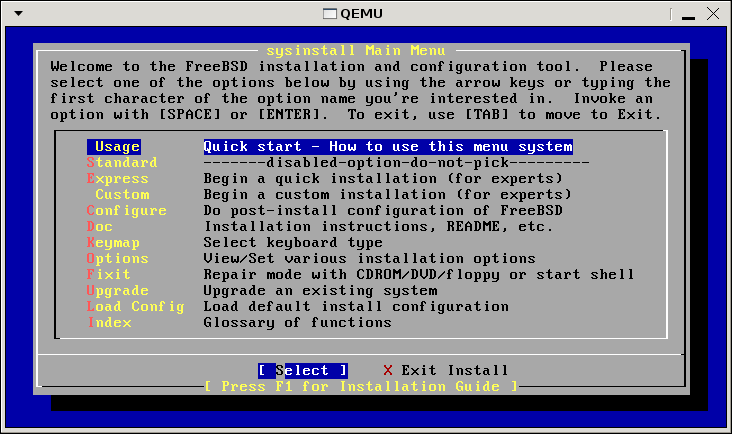
\includegraphics[width=\hsize]{image200708/kfreebsd-install-0.png}
 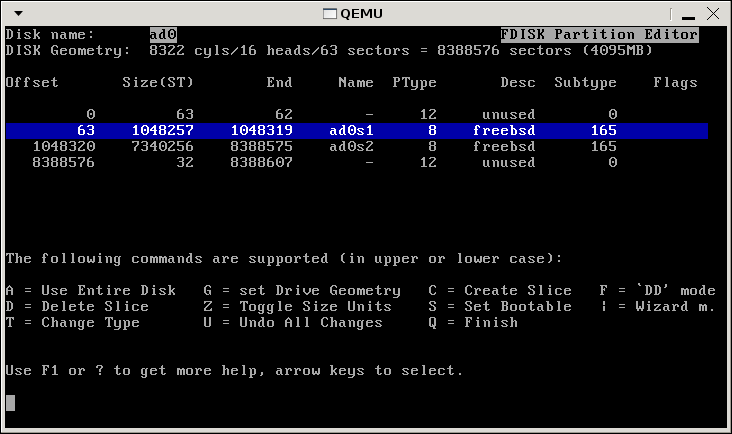
\includegraphics[width=\hsize]{image200708/kfreebsd-install-1.png}
 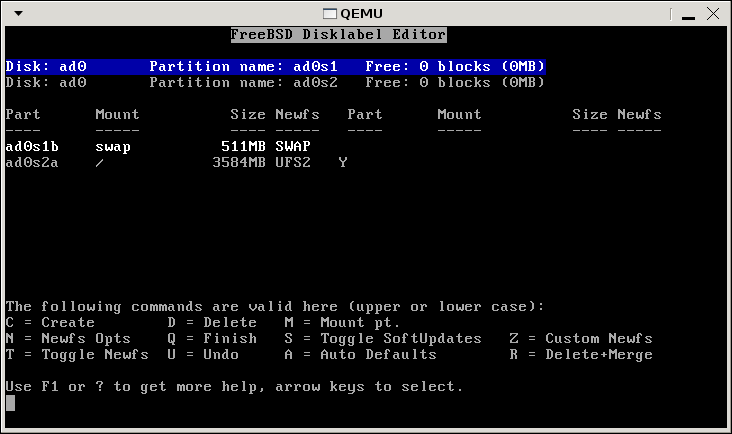
\includegraphics[width=\hsize]{image200708/kfreebsd-install-2.png}
 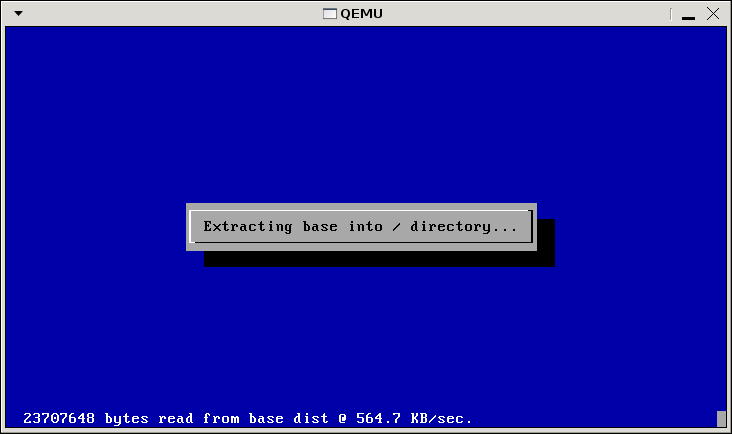
\includegraphics[width=\hsize]{image200708/kfreebsd-install-3.png}
 \end{multicols}
\caption{Debian GNU/kFreeBSD インストール画面}
\label{fig:kfreebsdinst}
\end{figure}

しばらく待つと alt-f3 で画面を切り替えろと表示されます。
debconf の質問に答つつインストールがつづきます。

\begin{figure}[H]
 \begin{center}
  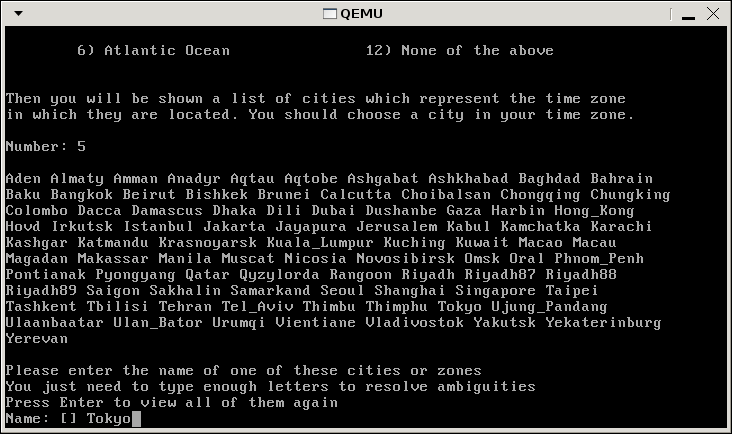
\includegraphics[width=0.5\hsize]{image200708/kfreebsd-install-4.png}
 \end{center}
 \caption{初期パッケージインストール・設定中}
 \label{fig:kfreebsdinst2}
\end{figure}

最後にリブートをするように指示されるので、そこで
qemu を一旦終了します。

ここで、 qemu を HDD イメージから起動するようにして実行します。

\begin{commandline}
 qemu-system-x86_64 -hda f.cow -m 256 
\end{commandline}

起動すると、なぜだか root filesystem が read-only だからといろいろと失敗
します。
fsck が必要な場合の起動に不都合があるようです。
一旦 root でログインし、reboot コマンドでリブートしてみると root
filesystem を正常にマウントすることが出来るようです。

また、 /etc/network/interfaces がまったく設定されていない状態なので、ネットワー
クが使えない状態で起動してきますが dhclient を実行すればIPを取得して稼働
することも可能です。

\begin{commandline}
 dhclient ed0
\end{commandline}

\subsection{動いた!}

これで無事に Debian GNU/kFreeBSD の稼働が確認できました。
まだまだ完成度が至らない点が多いので、デバッグしほうだいです。

 \begin{figure}[H]
  \begin{center}
   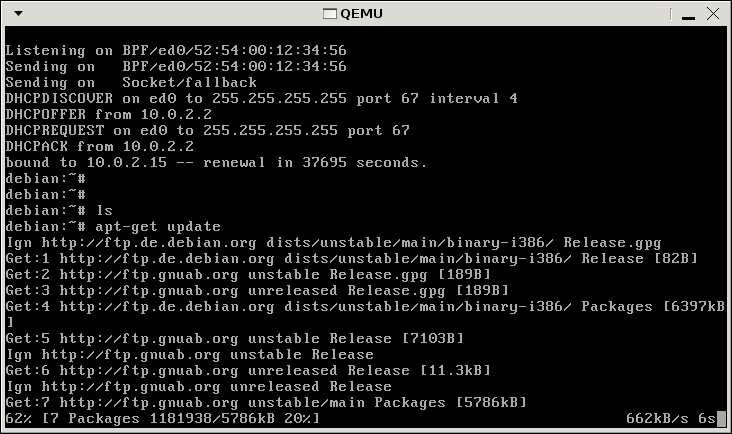
\includegraphics[width=0.5\hsize]{image200708/kfreebsd-install-5.png}
  \end{center}
  \caption{Debian GNU/kFreeBSD で apt-get してみました}
  \label{fig:kfreebsdaptget}
 \end{figure}
 
\dancersection{Exim 再発見}{小室 文}
\label{debianexim}
\index{exim}
\subsection{intro}
私達の日常ではメールは欠かせないコミュニケーションツールです。
それを実現する為に、導入される MTA( Mail Transfer Agent )は、どのソフトを使ったら
一番コストパフォーマンスが良いか、またどうやったら会社、グループ、個人のニーズに答える事が
出来るか、システム管理者は日夜頭を悩ましているはずです。そして一度導入したメールサーバーの
仕組みは、なかなか別の仕組みに乗り換えるのは、時間と費用がかかり、問題があったとしてもなか
なか移行しづらいという現状もあり、MTAを決めるのは人生でなかなか訪れない大決心の一つである
事は明白です。
MTA の一つ、Exim は Debian の Default MTA と呼ばれながらも、今や Postfix の人気に
すっかり影を潜めて過去の栄光に甘んじているのが現実です。
今日は Exim の歴史、利点・不利点、導入方法を御紹介します。 皆さんの MTA に選ばれなかった
としても、Exim はこういうパッケージなのか!と知って頂ければ幸いです。

\subsection{Eximとは}
Exim\footnote{Exim の名前の由来は EXperimental Internet Mailer (Exim)}
 とは、Unixもしくは Unix like なOSの上で動く Mail Transfer Agent です。Cygwin 
を使えば Windows の上でも動かす事が出来ます。Exim はケンブリッジ大学で 1995 年に Philip Hazel 
さんによって開発されました。\\

\subsection{Exim の歴史}
ケンブリッジ大学では、複数の MTA が動いていて(Sendmail, Smail, PP?などなど)、そんな環境
にうんざりしてたがどうかは不明ですが、Philip Hazel さんは Smail を拡張して MTA を大学のニーズ
に合わせて作ろうと試みました。しかし残念ながら、Smail 拡張はあっさり諦め、Hazel さんはスクラッチ
から MTA を作ろうと試みる事にしました。
その作業が、彼が所属した Computer Sceince の仲間に知れわたり、FTP サーバーを立てられ、配布され
るようになりました。
書いている途中で配布がされるようになった為、正式な Exim 0 もしくは 1 はリリースしていません
(少なくとも Hazel さんはリリース出来なかったと思っているようです)。\\
元々 Sendmail, Smail を触っていた Hazel さんは Sendmail に代わる MTA を作ろうと Exim 
を設計されています。 \\
\begin{tabular}[htb]{|l|l|} \hline
1995年?月 & Exim 開発開始\\ \hline
1995年11月 & 同僚が FTP サーバをつくりパッケージを配布始める。クチコミで広がる\\ \hline
1998年夏 & Perl の正規表現ライブラリーがなかったので作る(PCRE)\\ \hline
1999年3月 & コードネーム Slink の Debian 2.1 リリース。 Exim をディフォルト MTA として起用する \\ \hline
1999年9月 & ケンブリッジ大学で Exim の講座を開始する。 \\ \hline
2000年8月 & コードネーム potato の Debian 2.2 リリース\\ \hline
2002年7月 & コードネーム woody の Debian 3.0 リリース\\ \hline
2004年5月 & ケンブリッジ大学が Exim を正式にサポートすると宣言\\ \hline
2005年6月 & コードネーム sarge の Debian 3.1 リリース\\ \hline
2007年4月 & コードネーム etch のDebian 4.0 リリース\\ \hline
\end{tabular}

\subsection{Exim と Debian の関係}
\subsubsection{現在の Exim のメンテナー}
現在の Exim のメンテナーは
\begin{itemize}
\item Andreas Metzler  \url{ametzler@debian.org}
\item Marc Haber \url{mh@debian.org}
\end{itemize}
です。
Slink で Exim が搭載されるようになる前から、Sendmail や Smail から Exim へ移行を試みる人が沢山いた
ようです。
日本ではマニュアルの日本語化があまり進まず(現在も小数の人達が作業しているのみ)、Slink で Exim が搭載され
たので、移行した、という人が多かったようです。

\subsubsection{なぜ Exim は Debian の Default MTA になったのか!?}

\begin{tabular}[htb]{|l|l|} \hline
1996年09月 & Tim Cutt が Debian で Exim をパッケージとして提供する為に作業を始める \\ \hline
1997年05月 & Exim がunstable に入る by David Sewell \\ \hline
1999年03月 & Slink で Exim をディフォルト MTA として起用する。\\ \hline
\end{tabular}

当時は Postfix、Sendmail, Smail などがあったりましたが、ライセンス問題
\footnote{ライセンス形態:GNU General Public License (GPL)  ver2}
、機能の充実度合などがあり、
Debian の Defualt MTA になったようです。

\subsection{Exim と他の MTA の相違点}

\begin{tabular}[htb]{|l|ccc|} \hline
MTA&ライセンス形態 & メイン製作者 & リリース状態 \\ \hline
qmail&DJBライセンス&D. J. Bernstein& 1997年に出したっきり\\ \hline
Postfix&IBM Public License&Wietse Zweitze Venema&1997年にリリース後、都度都度にリリース \\ \hline
Exim&GPL&Philip Hazel&1995年にリリース後、都度都度リリース \\ \hline
\end{tabular}

\begin{itemize}
\item qmail
 \begin{itemize}
 \item 1997年からリリースされていない。IPv6 に対応してない。ライセンス形態、導入が難しい
 \item 大量メールを配信する場合、セキュリティー面
 \end{itemize}

\item Postfix
 \begin{itemize}
 \item Exim ほど機能の実装がない
 \item 移行が簡単、コミュニティーがアクティブ、日本でも使っているユーザーが多い(本も多い)
 \end{itemize}

\item Exim
 \begin{itemize}
 \item 日本語のマニュアルがない
 \item コミュニティーがアクティブ、Debian の Default MTA、ライセンス、ドキュメントが豊富(英語)
 \end{itemize}
\end{itemize}

\subsection{Exim の設定方法}
\subsubsection{既存パッケージ一覧}
現在の Debian の stable である etch には以下の Exim 向けパッケージが用意されています。

\begin{tabular}[htb]{|l|l|} \hline
exim4&Exim 4 を簡単にインストールする為にメタパッケージ\\ \hline
exim4-base&全 Exim 4 パッケージ支援パッケージ\\ \hline
exim4-config&Exim 4 設定用パッケージ \\ \hline
exim4-daemon-heavy&追加機能(exiscan-acl含む)を搭載しているデーモンパッケージ\\ \hline
exim4-daemon-light&簡易機能を搭載しているデーモンパッケージ\\ \hline
exim4-daemon-light-dbg&debug用\\ \hline
exim4-dbg&debug用\\ \hline
exim4-dev&ヘッダーファイル用の Exim 4 パッケージ \\ \hline
exim4-doc-html&Exim 4 の html 形式のドキュメントパッケージ\\ \hline
exim4-doc-info& Exim 4 の info 形式のドキュメントパッケージ\\ \hline
\end{tabular}

\subsubsection{インストール方法}

\begin{commandline}
aptitude install exim4 exim4-base exim4-config exim4-daemon-heavy
\end{commandline}
か
\begin{commandline}
aptitude install exim4 exim4-base exim4-config exim4-daemon-light
\end{commandline}
を実行します。

exim-config によって必要な情報入力はプロンプトが出るので指示に従います。 \\
\begin{enumerate}
\item 設定ファイルを分割するか、否か
\item メールの扱いについて(送信サーバの決定)
\item メールドメイン名について
\item 受けつけるメール送信元の IP 制限の決定( IPv6 対応)
\item Virtual Domain の下準備
\item オープンメールの設定
\item ローカルネットワークからの送信の決定
\item ダイヤルアップ時のDNS look upの決定
\item メール形式の決定(mbox/Maildir)
\end{enumerate}

\subsection{Exim のこれから}
 Philip Hazel さんは2007年2月8日付で、9月末に Exim から引退したいと申し出ましたが、
まだ決着はついていません。
すでに Exim を Hazel さんと同等に知っているメンテナーが世界中にいるので、肝はそれを統
括するマネージャーのような人を立てる、という事が大事になってくると思われます。\\
メインで動いている人達は Exim の新機能や、Exim をどのように運営、更新をしていくか 
\url{Exim-future@exim.org} という場所で会議をしようと試みています。\\
Debian では、 Exim 5 がリリースされるタイミングが現在もなお不透明な為、例え Lenny 
が近い未来リリースされる事があっても、その時に Exim 5 が間に合うとは保障出来ません。
日本では私がとりあえずマニュアルの翻訳をしようとExim ユーザー会を作ってみました。\\
\url{https://sourceforge.jp/projects/exim-jp}

\dancersection{あなたの知らないかもしれない apt-xxx}{岩松 信洋}
\label{aptxxx}
\index{apt-xxx}
\subsection{はじめに}
Debian ユーザーは apt がないと生きていけません。
apt-get はみんなが知っているコマンドですが、aptにはいろいろなコマンドが存在します。
今回はあまり知られていない apt-xxx について調べてみました。

\subsection{レベル 小}
勝手にレベルをつけていますが、レベル小 は一般ユーザの方なら知っておいて損はない
というものです。Debian 上での生活を楽にしてくれるかもしれません。

%\subsubsection{apt-howto}
% apt の使い方をまとめた Debian package です。
% 日本語向けのパッケージ apt-howto-ja もあります。

\subsubsection{apt-key}
\index{apt-key}
 apt の GPG鍵リングを制御するフロントエンドです。
 2006年から secure apt が導入された。secure apt は Debian アーカイブの信頼性を
 上げるため導入されたのですが、これには GPG が使われており、一般ユーザーにはちょっと
 難しいかもしれません。しかし、secure apt の GPG のキーは毎年変更されるので、今後使う
 ことがあるかもしれません。
 また、GUI で操作したい人のために 
 gui-apt-key\footnote{http://packages.debian.org/unstable/admin/gui-apt-key} 
 パッケージがあります。
 
\subsubsection{apt-spy}
\index{apt-spy}
 ネットワークの情報から最適な apt-line を生成することができるツールです。
 いまは cdn.debian.or.jp があるのでどうでもいいかんじです。

\subsubsection{auto-apt}
 auto-apt は世間では検索用のツールになっています。
 \footnote{ファイル検索用として apt-file というコマンドがあります。}
 \begin{commandline}
 % auto-apt upate
 % auto-apt search stdio.h
 usr/include/stlport/stdio.h     libdevel/libstlport5.1-dev
 usr/include/fcgi_stdio.h        libdevel/libfcgi-dev
 usr/include/H5FDstdio.h libdevel/libhdf5-lam-dev,libdevel/libhdf5-mpich-dev,libdevel/libhdf5-serial-dev
 usr/include/stdio.h     libdevel/libc6-dev
 \end{commandline}
 しかし、auto-apt は コマンド実行時に足りないファイルをパッケージをから探しだし、インストールしてくれるツールだったりします。
 \begin{commandline}
 # auto-apt run ./configure
 \end{commandline}
 

\subsubsection{cron-apt}
\index{cron-apt}
 apt-get update / apt-get uprade を cron で書いている人をたまに見かけますが、
 cron-apt を使えば、ログに apt の実行結果を残した設定が可能になります。
 似たような名前で apticron\footnote{http://packages.debian.org/unstable/admin/apticron}
 というパッケージがありますが、これはaptitude の cron-apt 版ではなく 
 セキュリティアップデート情報をメールで送信してくれるツールです。

\subsubsection{apt-proxy / apt-cacher}
\index{apt-proxy}
\index{apt-cacher}
 Debian パッケージのキャッシングプロキシを構築するパッケージです。
 例えば、家の中でマシンが数台あり、すべて sid だったとしましょう。特に設定を行ってない場合、
 各マシンは apt-get 毎に ミラーサーバーから Debian パッケージを取得します。
 これは無駄なので、1台だけ Debian パッケージをミラーサーバーから取得し、キャッシュし、他の
 マシンは対象のキャッシュしているパッケージを使ってアップデートを行うようにします。
 これを実現するためのパッケージが apt-proxy / apt-cacher です。
 \begin{figure}[h]
 \begin{center}
使用しない場合

 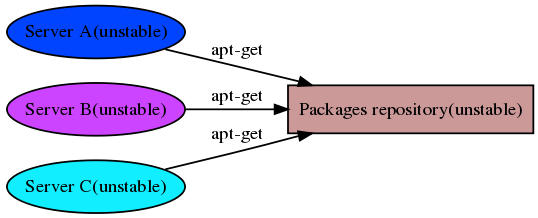
\includegraphics[width=10cm]{image200709/apt-proxy.png}
 \end{center}
 \end{figure}

 \begin{figure}[h]
 \begin{center}
使用した場合

 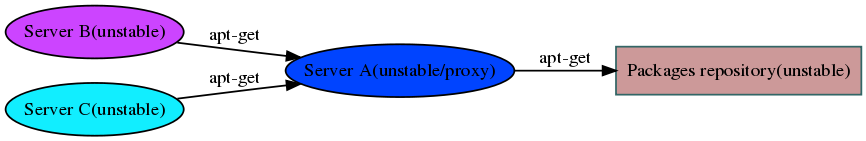
\includegraphics[width=15cm]{image200709/apt-proxy-e.png}
 \end{center}
 \end{figure}

%-------------------------
\subsection{レベル 中}
 一般ユーザーは知っていてもあまり役に立たないと思われる apt-xxx。
\subsubsection{apt-ftparchive}
\index{apt-ftparchive}
 Sources.gz / Packages.gz などのパッケージ情報用ファイルを作成するためのツール。
 自分で作ったパッケージを apt-line として公開したいときに使います。
\begin{commandline}
  % apt-ftparchive packages . | gzip -9 > Packages.gz 
  % apt-ftparchive sources . | gzip -9 > Sources.gz
  % apt-ftparchive release . > Release 
\end{commandline}

\subsubsection{apt-sortpkgs}
\index{apt-sortpkgs}
 Packages ファイル および Sources ファイルをソートします。apt-ftparchive で作成したものはソート
 されていなかったりするので、アルファベット順にソートするときに使います。
\begin{commandline}
 % apt-sortpkgs Packages > Packages.sort
\end{commandline} 

\subsubsection{apt-extracttemplates}
\index{apt-extracttemplates}
 Debian パッケージから設定とテンプレート情報を抽出するためのツールです。

\begin{commandline}
 % wget http://http.us.debian.org/debian/pool/main/x/xorg/xserver-xorg_7.3~rc1_all.deb
 % apt-extracttemplates xserver-xorg_7.3~rc1_all.deb
 % ls
 xserver-xorg.config.34261
 xserver-xorg.template.34260
\end{commandline}

\subsubsection{apt-build}
\index{apt-build}
 Debian で提供されているバイナリパッケージはあまり最適化されていません。
 人によっては自分の環境に合わせてチューニングしたり、製品に組み込んだりする場合もあります。
 apt-build は apt-get する感覚で環境に合わせてバイナリを作成をサポートするツールです。
 Debian パッケージをリビルドする場合は
 \begin{commandline}
 % apt-get update
 % apt-get source hello
 % cd hello-x.x
 % debuild -us -uc
 % sudo dpkg-i ../hello_xxxx.deb
 \end{commandline}
 という手順を踏みますが、apt-build の場合は
 \begin{commandline}
 % apt-get update
 % apt-build install hello
 \end{commandline}
 だけです。apt-build の設定ファイルは
 \begin{commandline}
 /etc/apt/apt-build.conf
 \end{commandline}
 にあり、
 \begin{commandline}
build-dir = /var/cache/apt-build/build
repository-dir = /var/cache/apt-build/repository
Olevel = -O3
march = -march=pentium2
mcpu = -mcpu=pentium2
options =
 \end{commandline}
 という設定になっています。例えば、自分の使っているマシンが i686 ではなく、Crusoe
 の場合には
\begin{commandline}
Olevel = 
-O2 -fomit-frame-pointer -fno-strict-aliasing -fno-common \ 
-pipe +-mpreferred-stack-boundary=2 -march=i686 -malign-functions=0 \
-malign-jumps=0 -malign-loops=0
\end{commandline}
とすればよいでしょう。

\subsubsection{apt-cross}
\index{apt-cross}
 Debian package を cross環境で使用できるように変換してインストールしてます。
 いままでは ダウンロードした Debian package を dpkg-cross で変換して
 インストールしていましたが、apt-cross を使うことのよって、手作業が減らすことが
 できます。

 \begin{figure}[h]
 \begin{center}
apt-cross を使用しない場合
 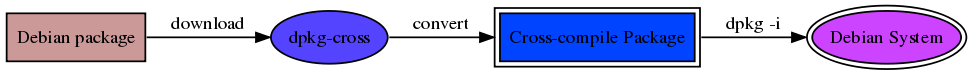
\includegraphics[width=16cm]{image200709/apt-cross.png}
 \end{center}
 \end{figure}

 \begin{figure}[h]
 \begin{center}
apt-cross を使用した場合

 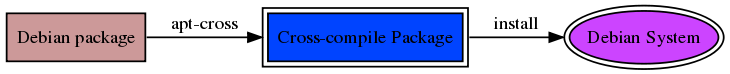
\includegraphics[width=12cm]{image200709/apt-cross-e.png}
 \end{center}
 \end{figure}

\subsubsection{apt-transport-https}
\index{apt-transport-https}
 apt はftp/http で取得できるのですが、このパッケージを使うことによって
 https 経由で apt を行うことができるようになります。
%------------------------- 
\subsection{レベル 高}
 知っていても使わないだろうと思われる apt-xxx.
 話のネタにはなるかもしれない。
\subsubsection{apt-zip}
\index{apt-zip}
 リムーバブルメディアの ZIP からの apt をサポートするためのツールです。
 同じようなツールで apt-cdrom がありますが、違いがいまいちわかりません。

\subsubsection{aptsh}
\index{aptsh}
 apt の操作をができる Shell.
\begin{commandline}
 % sudo aptsh
\end{commandline} 
 で shellが aptsh になります。試しに、
\begin{commandline}
 % ls
\end{commandline}
 を実行すると、インストール可能なパッケージ一覧が表示されます。
 
\subsection{まとめ}
今回はさわりだけを説明しました。今回の紹介で気になるapt-xxx がありましたら
詳細を説明していきたいと思っています。

\dancersection{DebTorrent に触ってみた}{山下 尊也}

\subsection{DebTorrentとは}
DebTorrentは、Debianパッケージを配布するためのプロトコルです。BitTorrent
と言うP2Pの技術を利用しています。具体的には、proxyでaptに渡しているみた
い。

BitTorrentの利点は、HTTPではパッケージのダウンロードが集中したときに、速度の低下
などが考えられますが、協力してダウンロードする事により、より多くのユーザ
に高速にファイルを配布出来ます。

調べてみたら、岩松さんが2007年の1月に東京エリア Debian 勉強会で
apt-torrentの話をしていたのですが、詳しく調べると、DebTorrentと
apt-torrentは違うみたいです。また、apt-torrentは2007年9月15日現在、公式
パッケージではありません。

\begin{commandline}
% aptitude show debtorrent
パッケージ: debtorrent
新規: yes
状態: インストールされていません
バージョン: 0.1.4.1
優先度: 任意
セクション: net
メンテナ: Cameron Dale <camrdale@gmail.com>
展開サイズ: 1217k
依存: python, python-support (>= 0.2), adduser
推奨: python-crypto, apt-transport-debtorrent
提案: python-psyco
提供: python-debtorrent
説明: bittorrent proxy for downloading Debian packages
 DebTorrent is a proxy for downloading Debian packages files with APT. It will
 download any needed packages from other DebTorrent peers in a bittorrent-like
 manner, and so reduce the strain on the Debian mirrors. 
 
 The DebTorrent client runs as a daemon, automatically started on bootup, and
 listens for requests from APT for files. Any non-package files are downloaded
 and served to APT similarly to other proxying software (e.g. apt-proxy,
 apt-cacher, and approx). The configuration is very simple, and only involves
 prepending a server and port to your current sources.list files (similar to
 apt-cacher). 
 
 When downloading package files, the DebTorrent client will try to use any other
 DebTorrent clients it can find to download from. This will use the uploading
 bandwidth of other peers, while reducing the demand on the Debian mirror
 network. However, if a package cannot be found on any peers, DebTorrent will
 fall back to downloading from a mirror to ensure all packages are downloaded. 
 
 Homepage: http://debtorrent.alioth.debian.org/
\end{commandline}

\newpage

\subsection{DebTorrentを用いてダウンロード}
\begin{enumerate}
 \item DebTorrentをインストールします。
       aptitude install debtorrent
 \item /etc/apt/sources.list を修正します。localhost:9988/cdn.debian.or.jp のようにする。

       ポートはフォルトでは、9988を利用しています。
       /etc/debtorrent/debtorrent-client.conf
       を変更する事で、ポート番号を変える事が出来ます。
 \item 後は、aptitude と一緒で、aptitude update
 \item aptitude install {\it packagename} でインストール出来ます。
\end{enumerate}

\begin{commandline}
# cat /etc/apt/sources.list
deb http://localhost:9988/cdn.debian.or.jp/debian/ sid main contrib non-free
\end{commandline}

\subsection{実際にやってみる}

残念ながら、Python 2.3以上でないと動かないため、etchでの利用は難しいと思
います。また、Q\&Aを読んでいると、experimentalを2007年9月15日現在、サポートしていないようで
す。

\begin{commandline}
# time apt-get source linux-source-2.6.22
Reading package lists... Done
Building dependency tree       
Reading state information... Done
Need to get 58.3MB of source archives.
Get:1 http://localhost sid/main linux-2.6 2.6.22-4 (dsc) [4832B]
Get:2 http://localhost sid/main linux-2.6 2.6.22-4 (tar) [57.4MB]                                                          
Get:3 http://localhost sid/main linux-2.6 2.6.22-4 (diff) [889kB]                                                          
Fetched 58.3MB in 26s (2165kB/s)                                                                                           
sh: dpkg-source: command not found
Unpack command 'dpkg-source -x linux-2.6_2.6.22-4.dsc' failed.
Check if the 'dpkg-dev' package is installed.
E: Child process failed

real    0m28.620s
user    0m7.280s
sys     0m0.728s
# 
\end{commandline}

実際に、この様にパッケージがある場所が見つかれば良いのですが、見つからない場合は、
いつまで経ってもダウンロードが始まりません。プロセスが死んだのかと不安に
なります。

しかし、見つかってしまえば結構な速度が出ます。
4回やった結果ですが最短は18秒。20秒、28秒、26秒と毎秒2MBほど出てるとなる
と嬉しくなります。

ちなみに、私は普段 cdn.debian.or.jp を使っていますが、同じ事を debtorrent を
使わずにやってみると、49秒かかりました。

ただ、今回の例では大きなファイルについてやっているので、小さなファイルで
実行したり、小さなファイルをたくさんダウンロードするとなると、httpの方が
速度が出ます。試しに、safe-upgradeをしてみましたが、ダウンロードに時間が
かなりの時間がかかり、話になりませんでした。

\subsection{まとめ}

私が考えたのは、security.debian.org は、stableやtestingのユーザに
いち早くセキュリティ修正されたパッケージを配っています。その際に、パッケー
ジの更新があれば、世界中のユーザからのアクセス集中により繋がりにくい状況に陥っ
たり、結果としてサーバダウンに繋がる事もあるので、DebTorrentはこのような
状況で使われたら良いのではないかと思ったのがきっかけでした。

ただ、今のstableには依存関係で導入が難しい事を考えると実際には、勧める事
は難しくなります。また、パッケージを送る側になる事も難しいでしょう。
しかし、おもしろい試みなので、今後も注目して、開発に期待したいと思います。


\newpage
\dancersection{live-helper}{岩松 信洋}
\label{live-helper}
\index{live-helper}
\subsection{live-helperとは}
live-helper は Debian の Live-CD / USBboot イメージを作成するための
ツールです。
作成するためのスクリプトが各種用意され、Live-CD の仕組みを知らない人でも容易
に Live-CD を作成することができます。

\subsection{コマンド}
live-helper はlh\_xxx という形式でコマンドが提供されています。
たくさんのコマンド\footnote{2007/11/02 現在で、67個}が用意されていますが、
基本的に使用するのは、
\begin{itemize}
  \item lh\_config
  \item lh\_build
  \item lh\_clean
\end{itemize}
です。他のコマンドは細かい設定を行うためや、内部処理で使用されます。

\subsection{雛型の作成}
まず、lh\_config コマンドを使って、Live-CD の雛形を作成します。
\begin{commandline}
% lh_config
\end{commandline}

{\bf lh\_config} 実行時にオプションを指定することにより、さまざまな設定を
行うことが可能です。
また、これらのオプションは環境変数としても指定することができます。
例えば、{\bf --union-filesystem} というオプションがあるのですが、この場合は
\begin{commandline}
LH_UNION_FILESYSTEM
\end{commandline}
として、設定することが可能です。
% 環境変数と、オプションで指定した場合の有線順位はどちらが高いか調べること

\subsection{作成された設定ファイルの説明}
lh\_config を実行した後、config ディレクトリ以下に以下のディレクトリが作成されます。
\begin{center}
\begin{tabular}{|c|c|}
\hline
ディレクトリ名 & 説明 \\ \hline \hline
binary & 作成される Live-CD イメージに関する設定が書かれています。\\ \hline
bootstrap & Live-CD 作成環境に関する設定が書かれています。\\ \hline
chroot & Live-CD のユーザーランドに関する設定が書かれています\\ \hline
common & live-helper の基本設定が書かれています。\\ \hline
source & source イメージに関する設定が書かれています。\\ \hline
\end{tabular}\\
\end{center}

これらの設定はテキストファイルになっています。なので、適当なエディタで編集可能ですが、
実際には {\bf lh\_config} コマンドを使い、設定ファイルを書き換えます。


\subsection{細かい設定方法}
live-helper は雛形を作成し、作成された各設定ファイルに追記することによって
細かいカスタマイズが可能になっています。以下にカスタマイズの方法について説明します。

\subsubsection{アーキテクチャの指定}

lh\_config の -a オプションを使用することによって、
作成する Live-CD イメージのアーキテクチャを指定することができます。

\begin{commandline}
% lh_config -a アーキテクチャ名
\end{commandline}

\subsubsection{ディストリビューションの指定}
lh\_config -d オプションを使用することにより、作成する Live-CD のディストリビューション
を指定することができます。

\begin{commandline}
% lh_config -d ディストリビューション名
\end{commandline}

\subsubsection{言語の指定}
lh\_config -l オプションを使用することにより、Live-CD で使用するデフォルトの言語を設定
することができます。
例えば、デフォルトの言語を日本語にする場合は
\begin{commandline}
% lh_config -l ja
\end{commandline}
とします。

\subsubsection{ブートローダーの指定}
lh\_config の --bootloader オプションを指定することにより、Live-CD で使用する
ブートローダーを指定することができます。

\begin{commandline}
% lh_config --bootloader grub
\end{commandline}

指定することができる ブートローダーは以下の3つです。
\begin{itemize}
\item grub
\item syslinux
\item yaboot
\end{itemize}

\subsubsection{作成するイメージの指定}
live-helperでは、
\begin{itemize}
\item iso 

ISO9660 イメージ
\item net

NET ブート用イメージ 
\item tar 

tar 形式でまとめたもの

\item usb-hdd

USBメモリやUSB-HDD で起動することができるイメージ

\end{itemize}
のイメージを作成することができます。

lh\_config の --binary-images\footnote{-b でも可能} 
オプションを指定することにより、作成するイメージを指定することができます。

\begin{commandline}
% lh_config --binary-images iso
\end{commandline}

\subsubsection{bootstrap および live-image 内で使用する apt-line の変更方法}
live-helper で使用する apt-line は
\begin{itemize}
\item Live-CD 作成に使用する apt-line
\item Live-CD 内の /etc/apt/sources.list に書き込まれる apt-line
\end{itemize}
の2種類があります。

これらは特に指定しない場合、
\begin{commandline}
http://ftp.debian.org/debian/
\end{commandline}
が指定されています。

変更する場合は {\bf lh\_config} コマンドを利用して変更します。
その他に以下の オプションを指定することによって各々の apt-line を変更する事ができます。

\begin{itemize}
\item --mirror-bootstrap-security URL

Live-CD 作成時に使用する セキュリティアップデート向け apt-line を設定します。 
\item --mirror-bootstrap URL

Live-CD 作成時に使用する apt-line を設定します。
\item -m \verb+|+ --mirror-binary-security URL

Live-CD 内で設定される、セキュリティアップーデート向け apt-line を設定します。
\item --mirror-binary URL

Live-CD 内で設定される、 apt-line を設定します。
\end{itemize}


\subsubsection{Debian パッケージの追加}
Live-CD に Debian Project で配布されているパッケージを追加したい場合は、
\begin{commandline}
lh_config --packages "パッケージ名"
\end{commandline}
を実行します。パッケージ名のところは、スペースで区切り、複数パッケージを指定することが可能です。

この方法でパッケージの追加を行った場合、再度実行してしまうと、上書きされてしまうためパッケージの
追加ができません。\footnote{エディタで編集すれば対応できますが。}

複数パッケージの追加や、パッケージの種類によって管理したい場合は
\begin{commandline}
config/chroot_local-packageslists/
\end{commandline}
ディレクトリに適当なファイルを作成し、パッケージ名を列挙します。
例えば、 bluetooth
\footnote{http://packages.debian.org/sid/bluetooth} メタパッケージを追加したい場合は、

\begin{commandline}
% cat config/chroot_local-packageslists/bluetooth
# bluetooth packages
bluetooth
\end{commandline}
として、パッケージ名をファイルに列挙します。

ファイル名は管理しやすい名前にしておくといいでしょう。

\subsubsection{オリジナル Debian パッケージの追加}

自分で作成した Debian パッケージや オリジナルのパッチを当てた Debian
パッケージは以下の方法で Live-CD に追加することができます。

まず、自分で作成したパッケージ用のレポジトリを作成します。
次に
\begin{commandline}
config/chroot_sources/適当なファイル名.bootstrap
\end{commandline}
を作成し、作成した レポジトリを apt-line として追記します。

\begin{commandline}
config/chroot_local-packageslists/
\end{commandline}
に適当なファイルを作成し、追加したいパッケージ名を書きます。

これにより、Live-CD 作成時に 作成した apt-line からパッケージがダウンロード
され、インストールされます。

作成したapt-line を Live-CD にも追加する場合は
\begin{commandline}
config/chroot_sources/適当なファイル名.binary
\end{commandline}
を作成し、作成した レポジトリを apt-line として追記します。

\subsubsection{apt-line を使わない Debian Package の追加方法}
\begin{commandline}
config/chroot_local-packages/
\end{commandline}
ディレクトリに Debian パッケージをコピーします。
コピーしておくことにより、自動的にLive-CD 内にインストールされます。
依存関係は解決してないので、必要なパッケージは別途 apt を使ってインストール
するように設定しておく必要があります。

\subsubsection{すでに用意されているパッケージリスト}
live-helper ではまとまった環境がパッケージリストとして用意されています。
これらを使用することによって、ある程度容易に Live-CD を作成することが
できるようになっています。
パッケージリストは
\begin{commandline}
/usr/share/live-helper/lists/
\end{commandline}
にあり、これらを利用することが可能です。
これらのリストを利用するには、{\bf lh\_config} オプションの {\bf --packages-lists | -p} 
を使用します。
gnome-desktop ベースの Live-CD を作成する場合、
\begin{commandline}
% lh_config -p gnome-desktop
\end{commandline}
とします。

\subsection{ホスト名を変更する}
Live-CD のホスト名を変更するには、
lh\_config の --hostname オプションを使用します。
\begin{commandline}
% lh_config --hostname myhostname
\end{commandline}
を実行し、設定したいホスト名を指定します。

\subsection{ユーザー名を変更する}
Live-CD に新しいユーザを追加するには、
lh\_config の --username オプションを使用します。
\begin{commandline}
% lh_config --username myname
\end{commandline}
を実行し、追加したいユーザ名を指定します。
パスワードは{\bf live}になっています。

\subsubsection{パッケージ化されていないソフトウェアの追加方法}
アイコンや簡単なスクリプトをパッケージ化せず、Live-CD にインストールしたい
場合があります。
この場合は、
\begin{commandline}
chroot_local-includes
\end{commandline}
ディレクトリに{\b content}ディレクトリを作成し、この中にファイルを追加します。
例えば、usr/bin/に hello\_world というプログラムを追加したい場合は
\begin{commandline}
chroot_local-includes/content/usr/bin/hello_world
\end{commandline}
にコピーします。

\subsubsection{カーネル用パッケージの追加}

Debian で提供されているカーネル用パッケージをLive-CD に追加するには
lh\_config の --linux-packages オプションを使用します。
\begin{commandline}
% lh_config --linux-packages "追加したいパッケージ名"
\end{commandline}

追記ができず、上書きになってしまうため、パッケージを追加したい場合は
\begin{commandline}
config/chroot
\end{commandline}
ファイルの
\begin{commandline}
LH_LINUX_PACKAGES
\end{commandline}
の部分を編集するとよいでしょう。

\subsubsection{フック機能}
Live-CD イメージ作成に処理を入れたいときに使用します。

\begin{commandline}
config/chroot_local-hooks
\end{commandline}
ディレクトリにシェルスクリプトを入れることによって動作します。

例えば、bluetooth パッケージを Live-CD 内にインストールし、
起動時に有効にしたい場合は

\begin{commandline}
% cat config/chroot_local-hooks/enable-bluetooth.sh
#!/bin/sh -x
sed -ie 's/^BLUETOOTH_ENABLED=.*/BLUETOOTH_ENABLED=1/' /etc/default/bluetooth
\end{commandline}
というようなファイルを作成しておくと、 Live-CD 内でデフォルトで有効になっています。

\subsubsection{CDROM 起動時のsplash 画面を変更する}

\begin{commandline}
% lh_config --syslinux-splash FILENAME
\end{commandline}
として、ファイル名を指定します。

\subsubsection{GRUB 起動時のsplash 画面を変更する}

\begin{commandline}
% lh_config --grub-splash FILENAME
\end{commandline}
として、ファイル名を指定します

\subsubsection{インタラクティブモード}
live-helper では設定したあと、自動的に各イメージが作成されます。
イメージ作成途中で、操作をしたいとき、インタラクティブモードに設定しておくことにより
手動で細かい設定をすることが可能になります。

\begin{commandline}
% lh_config --interactive enable
\end{commandline}


\subsection{イメージの作成}
作成した設定でイメージを作成するためには

\begin{commandline}
# lh_build
\end{commandline}

を実行します。実行すると、イメージの作成を開始します。
再度イメージを作成する場合は、
\begin{commandline}
#lh_clean
\end{commandline}
を実行し、キャッシュをクリアしてから行います。

\subsection{GUIを使った作成方法}
live-helper は基本的に提供されているスクリプトを駆使して、イメージを作成しますが、
GUI で作成するためのフロントエンドとして、live-magic というものが提供されています。
簡単な使い方を説明します。

\subsubsection{live-magic の起動}

\begin{commandline}
% sudo apt-get install live-magic
\end{commandline}
でインストールし、起動します。

\begin{multicols}{2}
 起動した直後の画面を右に示します。

 \begin{figure}[H]
 \begin{center}
  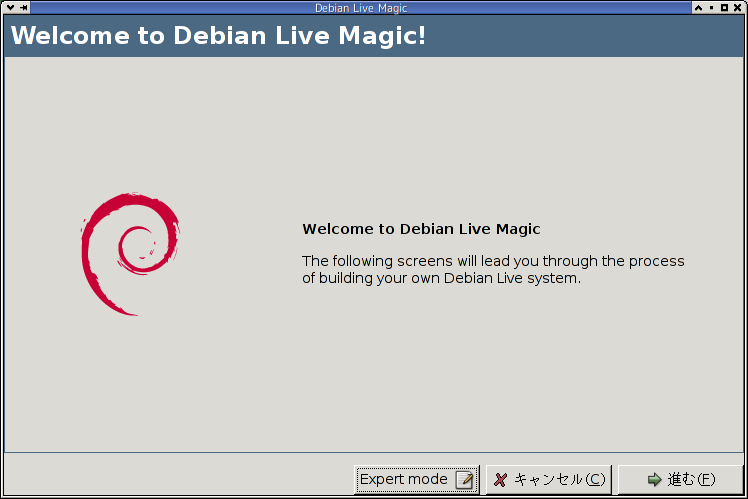
\includegraphics[width=1\hsize]{image200711/live-magic00.png}
 \end{center}
 \caption{live-magic 起動画面}
 \label{live-magic00}
 \end{figure}
\end{multicols}


\subsubsection{基本システムの選択}
次に基本システムを選択します。選択可能なシステムは以下の通りです。

\begin{multicols}{2}
 \begin{itemize}
 \item Gnome
 \item KDE
 \item XFCE
 \item non-Desktop
 \item システム復旧用 
 \end{itemize}

 \begin{figure}[H]
 \begin{center}
  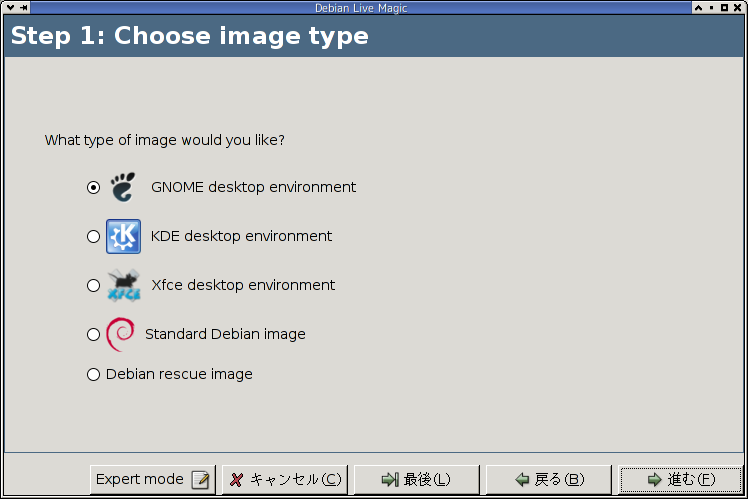
\includegraphics[width=1\hsize]{image200711/live-magic01.png}
 \end{center}
 \caption{live-magic 基本システムの選択}
 \label{live-magic01}
 \end{figure}
\end{multicols}

\subsubsection{作成イメージの選択}
次に作成するイメージを選択します。選択可能なイメージは以下の通りです。

\begin{multicols}{2}
 \begin{itemize}
 \item CD-ROM イメージ
 \item HDD イメージ
 \item NFS イメージ 
 \end{itemize}

 \begin{figure}[H]
 \begin{center}
  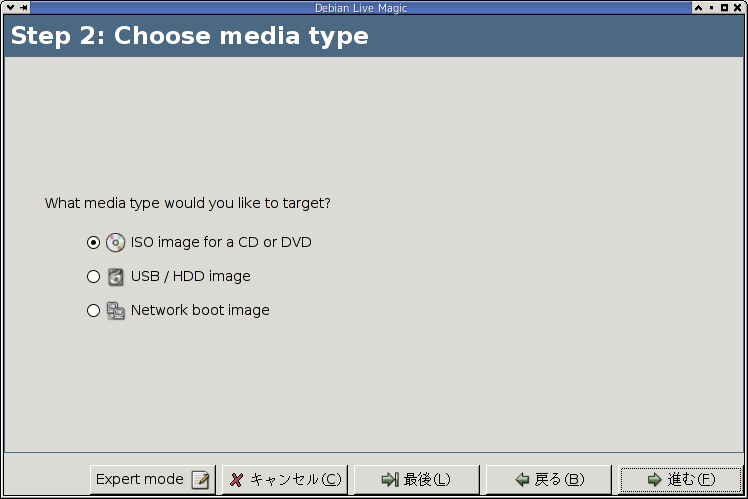
\includegraphics[width=1\hsize]{image200711/live-magic02.png}
 \end{center}
 \caption{live-magic 作成イメージの選択}
 \label{live-magic02}
 \end{figure}
\end{multicols}

\subsubsection{アーキテクチャの選択}
次に対象のアーキテクチャを選択します。選択可能なアーキテクチャは以下の通りです。

\begin{multicols}{2}
 \begin{itemize}
 \item i386
 \item powerpc
 \item amd64 
 \end{itemize}

 \begin{figure}[H]
 \begin{center}
  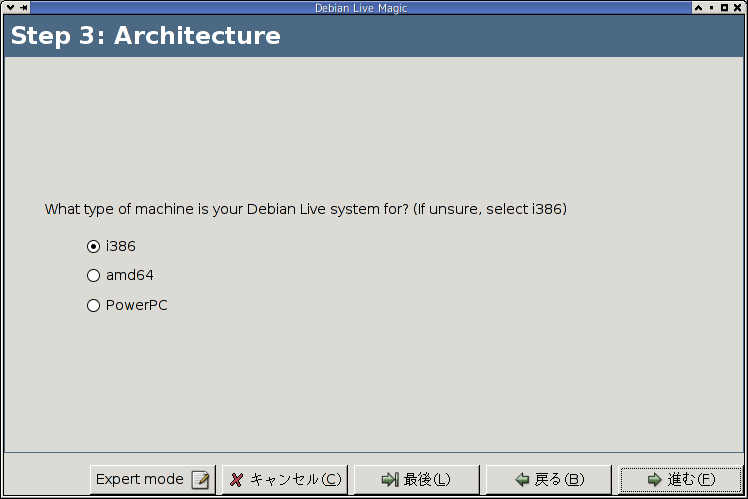
\includegraphics[width=1\hsize]{image200711/live-magic03.png}
 \end{center}
 \caption{live-magic アーキテクチャの選択}
 \label{live-magic03}
 \end{figure}
\end{multicols}

\subsubsection{ミラーサーバーの選択}
\begin{multicols}{2}
 次にミラーサーバーを選択します。

 \begin{figure}[H]
 \begin{center}
  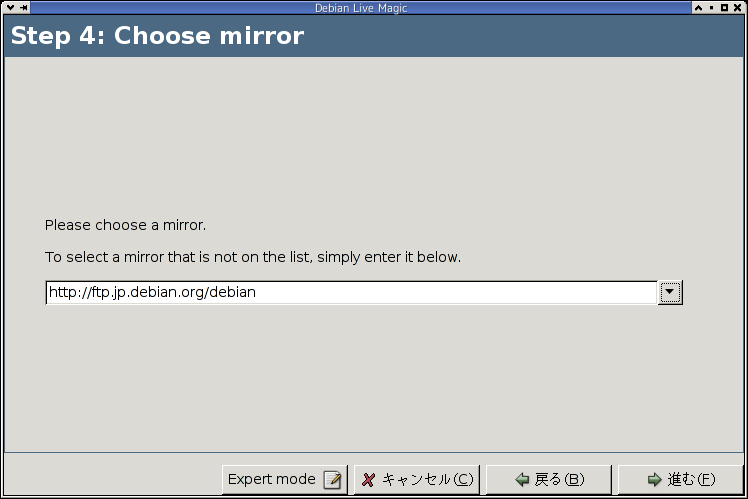
\includegraphics[width=1\hsize]{image200711/live-magic04.png}
 \end{center}
 \caption{live-magic ミラーサーバーの選択}
 \label{live-magic04}
 \end{figure}
\end{multicols}

\subsubsection{イメージ作成実行}
\begin{multicols}{2}
 適用ボタンを押すと、イメージ作成を実行します。

 \begin{figure}[H]
 \begin{center}
  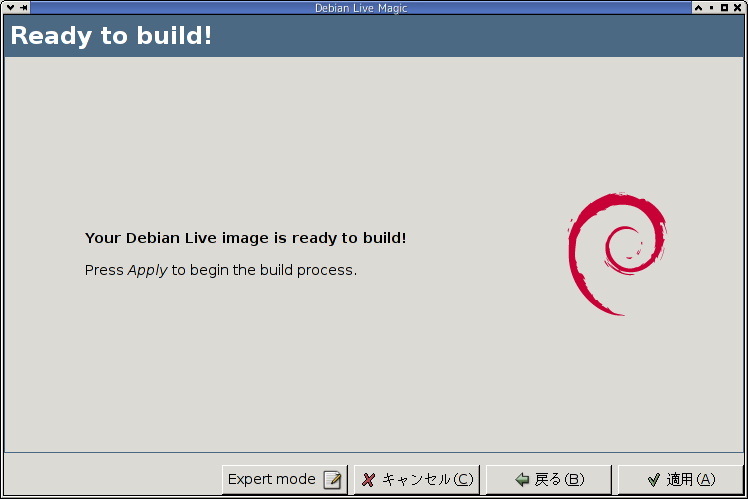
\includegraphics[width=1\hsize]{image200711/live-magic05.png}
 \end{center}
 \caption{live-magic イメージ作成実行}
 \label{live-magic05}
 \end{figure}
\end{multicols}


\subsubsection{rootパスワード要求}

\begin{multicols}{2}
 一般ユーザーで実行した場合、 rootのパスワードを要求されます。

 \begin{figure}[H]
 \begin{center}
  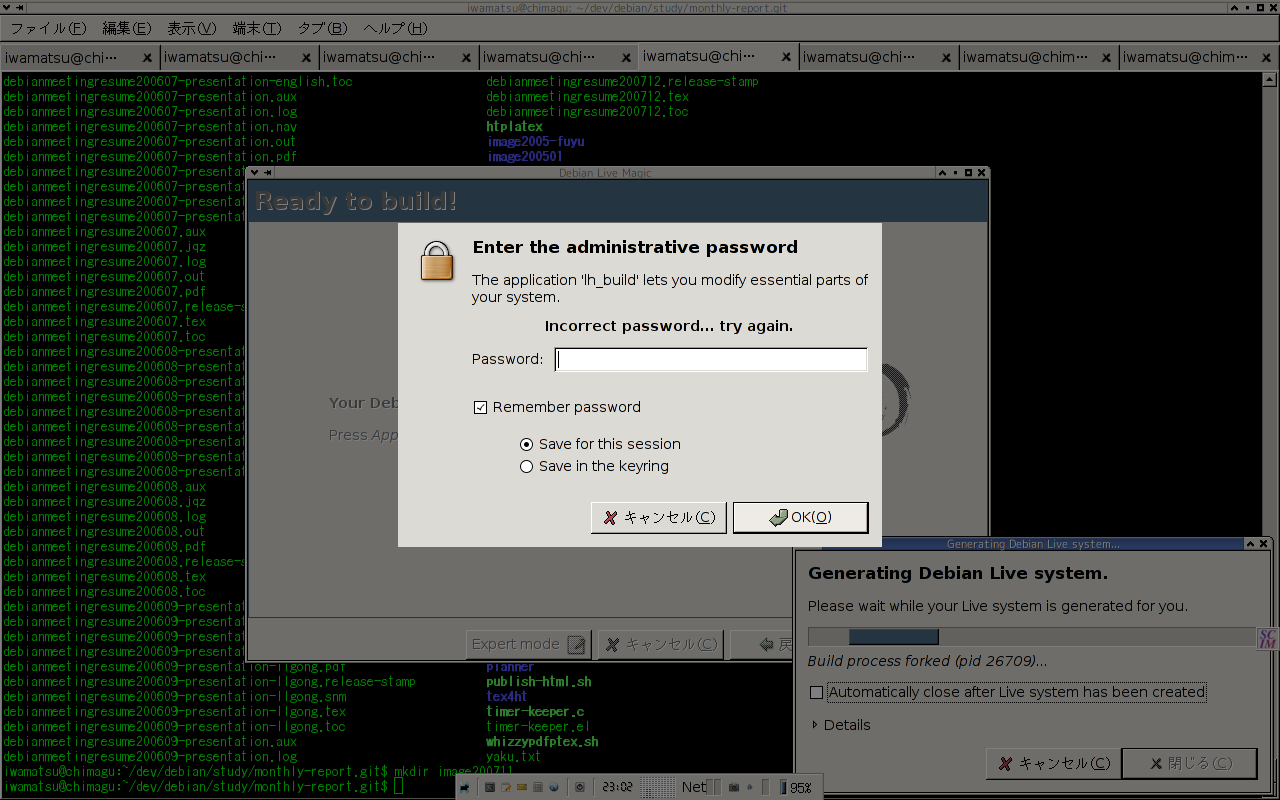
\includegraphics[width=1\hsize]{image200711/live-magic06.png}
 \end{center}
 \caption{live-magic rootパスワード要求画面}
 \label{live-magic06}
 \end{figure}
\end{multicols}

\subsubsection{作成中画面}

\begin{multicols}{2}
 イメージ作成中はプログレスバーが表示され、途中経過を確認することができます。

 \begin{figure}[H]
 \begin{center}
  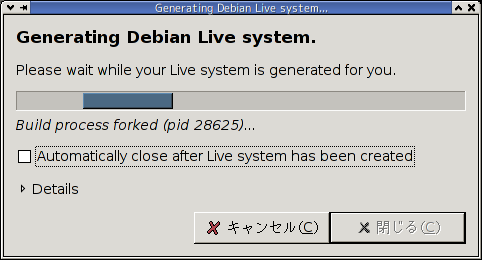
\includegraphics[width=1\hsize]{image200711/live-magic07.png}
 \end{center}
 \caption{live-magic 作成中画面}
 \label{live-magic07}
 \end{figure}
\end{multicols}

\subsubsection{デバッグ方法}
動作確認やデバッグのために、毎回作成した CD/DVD ISO イメージを 焼いていると
時間もお金もかかりますので、作成した ISO イメージのデバッグ方法について簡単に説
明したいと思います。

デバッグ方法はいろいろありますが、自分はqemu\footnote{http://packages.debian.org/sid/qemu}を使って動作確認しています。
\begin{commandline}
# apt-get update
# apt-get install qemu
% qemu -cdrom binary.iso
\end{commandline}
qemu を使ったエミュレーション環境でデバッグすることにより、時間や CD-R 代の節約にもなります。
他の方法としては、VMWare,VirtualPC を使ったデバッグ方法なども考えられます。

\subsection{live-helper を使ってみて}
\subsubsection{Live-CDからのインストールのサポート}
現状、Live-CD からのインストールがサポートされていません。
HDDイメージを作成することはできますが、一般ユーザーには敷居が高いと考えています。
Live-CD が気に入ったなら、動作している PC にインストールが容易にできるようになれば
ユーザーは増えるのではないでしょうか。

\subsubsection{日本語環境のサポート}
live-helper には、ある程度の環境をまとめたものとして、
packages-selections というものが提供されています。
これに日本語環境もサポートに入れることによって、日本語対応の Live-CD 作成が容易
になると思います。

\subsubsection{live-magic の日本語化}
live-helper のフロントエンドである live-magic が英語のままなので、国際化をしたい
ところです。


\subsection{その他の情報}
live-helper の情報は以下のサイトから得ることができます。
\begin{enumerate}
\item live-helper 公式サイト \url{http://debian-live.alioth.debian.org/}
\item wiki.debian.org \url{http://wiki.debian.org}

\end{enumerate}

% kansai debian
% ohura-san
\dancersection{Debian パッケージの作り方(1) -- 20分で作る Debian パッケージ --}{大浦 真(Debian Project)}
%\dancersection{Debian パッケージの作り方(1)}{大浦 真(Debian Project)}

\subsection{はじめに}
\begin{description}
\item[テーマ] 人は何分で Debian パッケージを作ることができるのか。
  (説明をしながら)
\item[題材] GNU Hello (\url{http://www.gnu.org/software/hello/})
\end{description}

\subsection{手順}
\begin{enumerate}
\item 必要なパッケージのインストール。
  \begin{itemize}
  \item \textbf{build-essential}
  \item そのソフトウェアのビルドに必要なパッケージ。
  \item \textbf{dh-make}、\textbf{debhelper}、\textbf{devscripts}、
      \textbf{fakeroot}、\textbf{lintian}/\textbf{linda}
  \end{itemize}
\item パッケージを作りたいソフトウェアのアーカイブを用意し展開。
\item \texttt{dh\_make} でソースツリーの雛型を作成。
\item ひとまず \texttt{debuild} でパッケージを作ってみる。
\item うまくいかない場合は、ログや \texttt{./debian/rules} ファイルを確認。
\item うまくできた場合は、\texttt{./debian/} 以下のファイルを確認。
  \begin{itemize}
  \item \texttt{./debian/changelog}: Debian パッケージの更新履歴。
  \item \texttt{./debian/control}: Debian パッケージの情報。
    (依存関係や説明文)
  \item \texttt{./debian/copyright}: ソフトウェアのライセンスの説明。
  \item \texttt{./debian/*.ex}: 必要になるかもしれないファイルの雛型。
    必要なければそのまま削除。
  \end{itemize}
\item \texttt{lintian} コマンドの出力を確認し、修正。
\item インストール。
\end{enumerate}

\begin{itemize}
\item 生成されるファイル
\begin{description}
\item[\ttfamily{}*.orig.tar.gz] オリジナルのソースアーカイブ。
\item[\ttfamily{}*.diff.gz] オリジナルのソースと Debian ソースパッケージとの間の差分。
\item[\ttfamily{}*.dsc] Debian ソースパッケージの情報。
\item[\ttfamily{}*\_i386.deb] バイナリパッケージ。
\item[\ttfamily{}*\_i386.changes] Debian パッケージの情報と最新の変更履歴。
\item[\ttfamily{}*\_i386.build] \texttt{debuild} のログ。
\end{description}
\end{itemize}

\subsection{参考文献}

\begin{itemize}
\item 「入門 Debian パッケージ」(やまだあきら[著]、鵜飼 文敏[監修]) 技術評論社
  (ISBN-10: 477412768X)
\item Debian Project の Web ページ内の「Debian 開発者のコーナー」
  (\url{http://www.jp.debian.org/devel/})。
  特に、「Debian ポリシーマニュアル」「デベロッパーズリファレンス」
  「新規メンテナのためのガイド」
\end{itemize}

\dancersection{Debian パッケージの作り方(2) -- debian/rules を読む --}{大浦 真(Debian Project)}
\index{debian/rules}

\subsection{はじめに}

\begin{description}
\item[テーマ] \texttt{debian/rules} ファイルを読んでみる。
\item[題材] \texttt{hello-debhelper} パッケージのソースパッケージ。
  \texttt{debhelper} の簡単なサンプルになっている。
\end{description}

\subsection{debian/rules とは}

\begin{itemize}
\item Debian パッケージを作るための手続きを記述したファイル。
\item makefile になっている。
  \begin{itemize}
  \item 一行目は `\texttt{\#!/usr/bin/make -f}' となっていなければならない。
  \item 最低限、clean、binary、binary-arch、binary-indep、build の
    五つのターゲットを含んでいなければならない。
  \item 必須のターゲット以外は自由に利用していい。
  \end{itemize}
  \begin{description}
  \item[{\ttfamily{}build}] ソースパッケージの設定とコンパイルを行う
    ためのターゲット
  \item[{\ttfamily{}binary、binary-arch、binary-indep}]
    バイナリパッケージを作るためのターゲット。
    binary-arch は、アーキテクチャに依存したパッケージ、
    binary-indep は、アーキテクチャに依存しないパッケージを作る。
    binary はその両方のパッケージを作る。
  \item[{\ttfamily{}clean}] 
    バイナリパッケージの作成後、ソースパッケージを元の状態に戻すための
    ターゲット。
  \item[{\ttfamily{}install}]
    ソースパッケージのコンパイル後、規定の位置にファイルを
    置くためのターゲット。
    \texttt{build} ターゲットで作成されたファイルは一旦、
    \texttt{debian/\$(package)/} 以下にインストールされる。
  \item[{\ttfamily{}configure}] ソースパッケージの設定を行うための
    ターゲット。
  \item[{\ttfamily{}get-orig-source}] オリジナルのソースパッケージを
    取得するためのターゲット。
    あまり知られていない。
  \end{description}
\item それぞれのターゲットを実行するための手助けをする
  \texttt{debhelper} という一連のスクリプトがある。
  \begin{itemize}
  \item 全て \texttt{dh\_} で始まる名前の perl スクリプト。
  \item \texttt{debhelper(7)} にスクリプトの一覧がある。
  \end{itemize}
  \begin{description}
  \item[\ttfamily{}dh\_clean] ソースパッケージの中のいらないファイルを
    削除する。
  \item[\ttfamily{}dh\_installdirs] \texttt{debian/\$(package)/} 以下に
    必要なディレクトリを作成する。
  \item[\ttfamily{}dh\_installdocs、dh\_installchangelog]
    \texttt{usr/share/doc/} 以下にドキュメントや changelog を
    インストール。
  \end{description}
  などなど。
\end{itemize}


\subsection{参考文献}

\begin{itemize}
\item Debian Policy (\url{http://www.jp.debian.org/doc/debian-policy/})
  「4.9 Main building script: debian/rules」
\end{itemize}

\dancersection{Debian パッケージの作り方(3) -- dpatch の使い方 --}{大浦真(Debian Project)}
\index{dpatch}

\subsection{はじめに}
\begin{description}
\item[テーマ] Debian パッケージの patch 管理システムである dpatch を
  使ってみる。
\item[素材] \texttt{hello-debhelper} パッケージのソースパッケージ。
  メッセージを変更する patch を作ってみる。
\end{description}


\subsection{Debian パッケージと patch}

\begin{itemize}
\item Debian のソースパッケージは三つのファイルから出来ている。
  \begin{description}
  \item[\ttfamily{}*.orig.tar.gz] オリジナルのソースアーカイブ。
  \item[\ttfamily{}*.diff.gz] オリジナルのソースと
    Debian ソースパッケージとの間の差分。
  \item[\ttfamily{}*.dsc] Debian ソースパッケージの情報。
  \end{description}
\item debian/ 以下のファイルも含めて、オリジナルとの差分は全て
  .diff.gz にまとめられるので、
  Debian 側で patch を複数あてている場合は管理が面倒。
\item dpatch を使うと、patch を分割して管理することができる。
  オリジナルが更新された時の追随も簡単。
\item debian/patches/ 以下で patch をまとめて管理。
\item 移行に .orig.tar.gz の修正は不要。
\end{itemize}

\subsection{dpatch の使い方}

\begin{itemize}
\item debian/rules の修正
  \begin{itemize}
  \item 冒頭に \texttt{include /usr/share/dpatch/dpatch.make} を追加。
  \item \texttt{build} ターゲットで \texttt{patch} ターゲットが、
    \texttt{clean} ターゲットで
    \texttt{unpatch} ターゲットが実行されるように変更する。
  \end{itemize}
  \begin{screen}[5]
    \#!/usr/bin/make -f \\
    \hspace{4em}\ldots \\
    include /usr/share/dpatch/dpatch.make \\
    clean: unpatch \\
    \hspace{4em}\ldots \\
    install: build \\
    \hspace{4em}\ldots \\
    build: patch \\
    \hspace{4em}\ldots
  \end{screen}
\item debian/control の Build-Depends: に dpatch を追加。
\item \textsf{dpatch-convert-diffgz} を使うと \texttt{.diff.gz} の中の
  debian/* 以外のファイルに対する patch を抽出できる。
\item \textsf{dpatch-edit-patch} で patch を作成。
  \begin{screen}[5]
    \$ dpatch-edit-patch 01\_hello\_japan \\
    ( \ldots 自動的に /tmp 以下にコピーが作られ、新しいシェルが起動する。) \\
    ( \ldots ソースツリーを修正。) \\
    \$ exit \\
    \$ 
    ( \ldots debian/patches/ 以下に patch ができる。)
  \end{screen}
  既存の patch の編集もできる。
\item できた patch (上例では、debian/patches/01\_hello\_japan.dpatch) に
  適当なコメントを書いておく。
\item patch を debian/patches/00list に追加。
  ファイル名の .dpatch を除いた文字列を追加。
\item patch がきちんと適用できるかどうかは、
  \textsf{fakeroot ./debian/rules patch}、
  \textsf{fakeroot ./debian/rules unpatch} で確認できる。
\item \textsf{dpatch-list-patch} で patch の一覧を確認できる。
\end{itemize}

\subsection{類似のシステム}

\begin{itemize}
\item dbs: オリジナルのソースが .tar.gz の形でそのまま .orig.tar.gz に
  含まれる。移行には、.orig.tar.gz の修正が必要。
\item quilt
\end{itemize}

\subsection{参考文献}

\begin{itemize}
\item dpatchの利用方法
  (\url{http://www.netfort.gr.jp/~dancer/column/dpatch.html.ja})
\item dpatch(1), dpatch.make(7),
  /usr/share/doc/dpatch/examples/rules/rules.new.dh.gz
\item 「入門 Debian パッケージ」(やまだあきら[著]、鵜飼 文敏[監修]) 技術評論社
  (ISBN-10: 477412768X)
\end{itemize}


\dancersection{Debian パッケージの作り方(4) -- ライブラリ編 --}{大浦 真(Debian Project)}
\subsection{はじめに}

\begin{description}
\item[テーマ] ライブラリの Debian パッケージ作成を実演してみる。
  普通のパッケージよりも少し複雑。
\item[素材] \texttt{libhello} (``Hello, library world.'' と表示する
  関数 hello を提供するライブラリ)
\end{description}

\subsection{基本的な手順}

\begin{enumerate}
\item 必要なパッケージのインストール。
  \begin{itemize}
  \item \textbf{build-essential}
  \item そのソフトウェアのビルドに必要なパッケージ。
  \item \textbf{dh-make}、\textbf{debhelper}、\textbf{devscripts}、
      \textbf{fakeroot}、\textbf{lintian}/\textbf{linda}
  \end{itemize}
\item パッケージを作りたいソフトウェアのアーカイブを用意し展開。
\item \texttt{dh\_make} でソースツリーの雛型を作成。
\item ひとまず \texttt{debuild} でパッケージを作ってみる。
\item うまくいかない場合は、ログや \texttt{debian/rules} ファイルを確認。
\item うまくできた場合は、lintian の出力や
  \texttt{debian/} 以下のファイルを確認し、さらに修正。
\end{enumerate}


\subsection{ライブラリパッケージの作り方}


\begin{itemize}
\item ライブラリパッケージは、共有ライブラリ本体が含まれる
  パッケージ (\textbf{libhello0}) と開発用のファイルが含まれる
  パッケージ (\textbf{libhello-dev}) に分かれている。
\item ライブラリの場合も、\texttt{dh\_make} で雛型を作ることができるが
  そのままではパッケージができない。
\item \texttt{debian/control} の修正
  \begin{itemize}
  \item \texttt{dh\_make} の指示通り、`libhelloBROKEN' となっている
    部分を修正。
    この場合は、`libhello0' にする。
  \end{itemize}
\item \texttt{debian/rules} の修正
  \begin{itemize}
  \item `\$(MAKE) distclean' の行を
    `[ ! -f Makefile ] $||$ \$(MAKE) distclean' に変更。
  \item \texttt{dh\_install} に `--sourcedir=debian/tmp' というオプションを
    付ける必要がある
    \footnote{かつては \texttt{dh\_movefiles} というものがあったが、現在は
      使われていない。}。
  \item \texttt{dh\_makeshlibs} を有効にする。-V オプションを付ける。
    有効にすると、適切な \texttt{postinst}/\texttt{postrm} スクリプトが
    用意される。(install 時と remove 時に \texttt{ldconfig} が
    実行される。)
  \end{itemize}
\item その他
  \begin{itemize}
  \item \texttt{libhello1.dirs} と \texttt{libhello1.install} を
    \texttt{libhello0} に名前を変える。
  \item \texttt{libhello-dev.install} から \textbf{pkg-config} 関係を削除。
  \item 不要な \texttt{debian/*.ex} を削除。
  \end{itemize}
\end{itemize}


\subsection{共有ライブラリの名前}

\begin{itemize}
\item 共有ライブラリは、三つの名前を持つ。
  \begin{description}
  \item[soname] (\texttt{/usr/lib/libhello.so.0}):
    実行ファイルが参照する名前。ライブラリのインターフェイスが変更されると
    末尾の数字が変わる。
    Debian ではこの数字をパッケージ名に付加する。
  \item[real name] (\texttt{/usr/lib/libhello.so.0.0.0}):
    ライブラリの実体。soname はこのファイルへのシンボリックリンクになっている。
  \item[linker name] (\texttt{/usr/lib/libhello.so}):
    ライブラリを利用するプログラムをコンパイルするときに参照する名前。
  \end{description}
\end{itemize}

\subsection{参考文献}

\begin{itemize}
\item \url{http://www.linux.or.jp/JF/JFdocs/Program-Library-HOWTO/}
  「Program Library HOWTO」(JF)
\item \url{http://www.netfort.gr.jp/~dancer/column/libpkg-guide/libpkg-guide.html}
  「Debian Library Packaging guide」
\end{itemize}


\subsection{サンプル}


\begin{itembox}{\texttt{libhello.c}}
\begin{verbatim}
#include <stdio.h>

void hello(void) {
        printf("Hello, library world.\n");
}
\end{verbatim}
\end{itembox}

\begin{itembox}{\texttt{libhello.h}}
\begin{verbatim}
void hello(void);
\end{verbatim}
\end{itembox}

\begin{itembox}{\texttt{demo\_use.c}}
\begin{verbatim}
#include "libhello.h"

int main(void) {
        hello();
        return 0;
}
\end{verbatim}
\end{itembox}

\newpage

\dancersection{HP ML350G5 Debian etch 動作確認}{上川 純一}
\label{ml350g5}
\index{ML350G5}

\subsection{サーバ}

HP ML350G5 は Intel Xeon CPUを搭載している
Debian 4.0 (etch) が稼働することがハードウェアベンダ、およびDebianプロジェ
クトの有志によって確認されているサーバ
\footnote{HP の ProLiant のDebian GNU/Linux 対応ページ:
\url{http://www.hp.com/go/debian}}
\footnote{Debian の ProLiant on Debian ページ:
\url{http://wiki.debian.org/HP/ProLiant}}
です。
今回利用したサーバには300GBのSASディスクが6本搭載されていました。

\subsection{インストール前の準備}

サーバの起動時に「F8」を押し、
ハードウェアRAID機能の設定を行います。
今回は一つのRAID5のボリューム(約1.5TB)としてOSに見せる設定にしました。

\subsection{インストール}

Debian installer でインストールします。今回はDebian GNU/Linux 4.0r1 DVD 
の1枚目を利用しました。ML350G5 は em64t 対応の Xeon のため、i386 でも 
amd64 でも動作します。今回は amd64 をインストールしました。

\subsection{デバイスの認識}

各種デバイスは簡単に稼働します。
グラフィックカードは ati ドライバで動作します。
debconf で自動設定した値で適切な設定ファイルが出力されます。

\begin{commandline}
# dpkg-reconfigure xserver-xorg
\end{commandline}

\subsection{USB ストレージデバイスの認識}

手元にあった「Green house GH-UFD2GR」のUSBメモリで動作確認したところ、認
識しました。

dmesg は次のようになりました:

\begin{commandline}
 usb 6-6: new high speed USB device using ehci_hcd and address 4
 usb 6-6: configuration #1 chosen from 1 choice
 Initializing USB Mass Storage driver...
 scsi0 : SCSI emulation for USB Mass Storage devices
 usbcore: registered new driver usb-storage
 USB Mass Storage support registered.
 usb-storage: device found at 4
 usb-storage: waiting for device to settle before scanning
  Vendor: USBDisk   Model: FlashDisk         Rev: 1.00
  Type:   Direct-Access                      ANSI SCSI revision: 02
 usb-storage: device scan complete
 SCSI device sda: 4005000 512-byte hdwr sectors (2051 MB)
 sda: Write Protect is off
 sda: Mode Sense: 0b 00 00 08
 sda: assuming drive cache: write through
 SCSI device sda: 4005000 512-byte hdwr sectors (2051 MB)
 sda: Write Protect is off
 sda: Mode Sense: 0b 00 00 08
 sda: assuming drive cache: write through
 sda: sda1
 sd 0:0:0:0: Attached scsi removable disk sda
 FAT: utf8 is not a recommended IO charset for FAT filesystems, filesystem will be case sensitive!
\end{commandline}


df で確認しても認識されているのがわかります:

\begin{commandline}
# df -h /media/usbdisk/
Filesystem            Size  Used Avail Use% Mounted on
/dev/sda1             2.0G   76M  1.9G   4% /media/usbdisk
# df -T /media/usbdisk/
Filesystem    Type   1K-blocks      Used Available Use% Mounted on
/dev/sda1     vfat     2001888     76864   1925024   4% /media/usbdisk
\end{commandline}

\subsection{USB webcam の認識}

PlayStation2 用USBカメラ EyeToy を動作させてみました。ov51x-jpeg のデバイ
スドライバを認識させるためのドライバは残念ながらDebian 4.0 には含まれてい
ないので、最新のドライバをバックポートしてみました。

\begin{figure}[H]
\begin{center}
  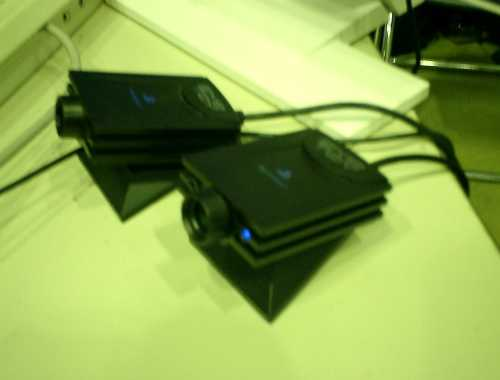
\includegraphics[width=0.5\hsize]{image200710/eyetoy.jpg}
\end{center}
\caption{EyeToy カメラ}
\label{eyetoy}
\end{figure}

%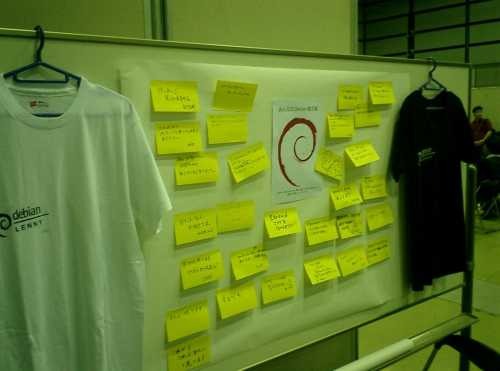
\includegraphics[width=0.5\hsize]{image200710/whiteboard.jpg}

まず、インストールされたカーネルでコンパイルするために必要なパッケージを
インストールします。

\begin{commandline}
apt-get install linux-headers-2.6.18-5-amd64 linux-kbuild-2.6.18 \
 linux-source-2.6.18
\end{commandline}

ov51x-jpeg のソースを取得して make コマンドでビルドできます。

\begin{commandline}
debian:/home/hoge/ov51x-jpeg# make 
make -C /lib/modules/2.6.18-5-amd64/build M=/home/hoge/ov51x-jpeg modules
make[1]: Entering directory `/usr/src/linux-headers-2.6.18-5-amd64'
  CC [M]  /home/hoge/ov51x-jpeg/ov51x-jpeg-core.o
  CC [M]  /home/hoge/ov51x-jpeg/ov511-decomp.o
  CC [M]  /home/hoge/ov51x-jpeg/ov518-decomp.o
  CC [M]  /home/hoge/ov51x-jpeg/ov519-decomp.o
  LD [M]  /home/hoge/ov51x-jpeg/ov51x-jpeg.o
  Building modules, stage 2.
  MODPOST
  CC      /home/hoge/ov51x-jpeg/ov51x-jpeg.mod.o
  LD [M]  /home/hoge/ov51x-jpeg/ov51x-jpeg.ko
make[1]: Leaving directory `/usr/src/linux-headers-2.6.18-5-amd64'
 
\end{commandline}

生成されたモジュールをあわせて insmod すれば ekiga で画面が見れるようになります。

\begin{commandline}
insmod v4l1-compat.ko
insmod v4l2-common.ko
insmod videodev.ko
insmod ov51x-jpeg.ko
\end{commandline}

\subsection{謝辞}

OSC Tokyo/Fall 2007 Debian ブースにて本作業を行いました。
サーバは日本HPからお借りしました。

\begin{figure}[H]
\begin{center}
  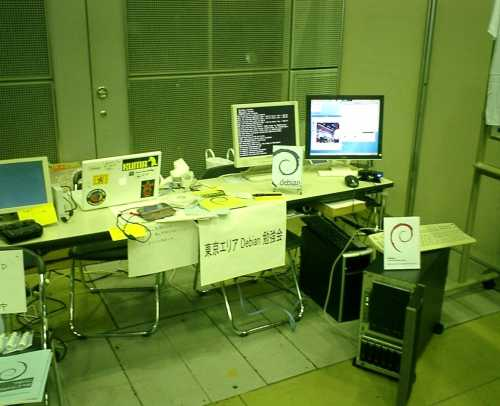
\includegraphics[width=0.5\hsize]{image200710/booth.jpg}
\end{center}
\caption{検証時のブースの様子}
\label{fig:oscfalldebbooth}
\end{figure}
\subsection{付録}

\subsubsection{デバイス接続}

\begin{commandline}
# lspci 
00:00.0 Host bridge: Intel Corporation 5000Z Chipset Memory Controller Hub (rev b1)
00:02.0 PCI bridge: Intel Corporation 5000 Series Chipset PCI Express x8 Port 2-3 (rev b1)
00:03.0 PCI bridge: Intel Corporation 5000 Series Chipset PCI Express x4 Port 3 (rev b1)
00:04.0 PCI bridge: Intel Corporation 5000 Series Chipset PCI Express x4 Port 4 (rev b1)
00:05.0 PCI bridge: Intel Corporation 5000 Series Chipset PCI Express x4 Port 5 (rev b1)
00:10.0 Host bridge: Intel Corporation 5000 Series Chipset Error Reporting Registers (rev b1)
00:10.1 Host bridge: Intel Corporation 5000 Series Chipset Error Reporting Registers (rev b1)
00:10.2 Host bridge: Intel Corporation 5000 Series Chipset Error Reporting Registers (rev b1)
00:11.0 Host bridge: Intel Corporation 5000 Series Chipset Reserved Registers (rev b1)
00:13.0 Host bridge: Intel Corporation 5000 Series Chipset Reserved Registers (rev b1)
00:15.0 Host bridge: Intel Corporation 5000 Series Chipset FBD Registers (rev b1)
00:16.0 Host bridge: Intel Corporation 5000 Series Chipset FBD Registers (rev b1)
00:1c.0 PCI bridge: Intel Corporation 631xESB/632xESB/3100 Chipset PCI Express Root Port 1 (rev 09)
00:1d.0 USB Controller: Intel Corporation 631xESB/632xESB/3100 Chipset UHCI USB Controller #1 (rev 09)
00:1d.1 USB Controller: Intel Corporation 631xESB/632xESB/3100 Chipset UHCI USB Controller #2 (rev 09)
00:1d.2 USB Controller: Intel Corporation 631xESB/632xESB/3100 Chipset UHCI USB Controller #3 (rev 09)
00:1d.3 USB Controller: Intel Corporation 631xESB/632xESB/3100 Chipset UHCI USB Controller #4 (rev 09)
00:1d.7 USB Controller: Intel Corporation 631xESB/632xESB/3100 Chipset EHCI USB2 Controller (rev 09)
00:1e.0 PCI bridge: Intel Corporation 82801 PCI Bridge (rev d9)
00:1f.0 ISA bridge: Intel Corporation 631xESB/632xESB/3100 Chipset LPC Interface Controller (rev 09)
00:1f.1 IDE interface: Intel Corporation 631xESB/632xESB IDE Controller (rev 09)
01:03.0 VGA compatible controller: ATI Technologies Inc ES1000 (rev 02)
01:04.0 System peripheral: Compaq Computer Corporation Integrated Lights Out Controller (rev 03)
01:04.2 System peripheral: Compaq Computer Corporation Integrated Lights Out  Processor (rev 03)
01:04.4 USB Controller: Hewlett-Packard Company Unknown device 3300
01:04.6 Serial bus controller [0c07]: Hewlett-Packard Company Unknown device 3302
02:00.0 PCI bridge: Broadcom EPB PCI-Express to PCI-X Bridge (rev c3)
03:00.0 Ethernet controller: Broadcom Corporation NetXtreme II BCM5708 Gigabit Ethernet (rev 12)
04:00.0 PCI bridge: Intel Corporation 6311ESB/6321ESB PCI Express Upstream Port (rev 01)
04:00.3 PCI bridge: Intel Corporation 6311ESB/6321ESB PCI Express to PCI-X Bridge (rev 01)
05:00.0 PCI bridge: Intel Corporation 6311ESB/6321ESB PCI Express Downstream Port E1 (rev 01)
05:01.0 PCI bridge: Intel Corporation 6311ESB/6321ESB PCI Express Downstream Port E2 (rev 01)
12:00.0 PCI bridge: Broadcom EPB PCI-Express to PCI-X Bridge (rev b4)
13:04.0 PCI bridge: Broadcom HT1000 PCI/PCI-X bridge (rev b2)
13:08.0 RAID bus controller: Hewlett-Packard Company Unknown device 3238

# lspci -n 
00:00.0 0600: 8086:25d0 (rev b1)
00:02.0 0604: 8086:25f7 (rev b1)
00:03.0 0604: 8086:25e3 (rev b1)
00:04.0 0604: 8086:25e4 (rev b1)
00:05.0 0604: 8086:25e5 (rev b1)
00:10.0 0600: 8086:25f0 (rev b1)
00:10.1 0600: 8086:25f0 (rev b1)
00:10.2 0600: 8086:25f0 (rev b1)
00:11.0 0600: 8086:25f1 (rev b1)
00:13.0 0600: 8086:25f3 (rev b1)
00:15.0 0600: 8086:25f5 (rev b1)
00:16.0 0600: 8086:25f6 (rev b1)
00:1c.0 0604: 8086:2690 (rev 09)
00:1d.0 0c03: 8086:2688 (rev 09)
00:1d.1 0c03: 8086:2689 (rev 09)
00:1d.2 0c03: 8086:268a (rev 09)
00:1d.3 0c03: 8086:268b (rev 09)
00:1d.7 0c03: 8086:268c (rev 09)
00:1e.0 0604: 8086:244e (rev d9)
00:1f.0 0601: 8086:2670 (rev 09)
00:1f.1 0101: 8086:269e (rev 09)
01:03.0 0300: 1002:515e (rev 02)
01:04.0 0880: 0e11:b203 (rev 03)
01:04.2 0880: 0e11:b204 (rev 03)
01:04.4 0c03: 103c:3300
01:04.6 0c07: 103c:3302
02:00.0 0604: 1166:0103 (rev c3)
03:00.0 0200: 14e4:164c (rev 12)
04:00.0 0604: 8086:3500 (rev 01)
04:00.3 0604: 8086:350c (rev 01)
05:00.0 0604: 8086:3510 (rev 01)
05:01.0 0604: 8086:3514 (rev 01)
12:00.0 0604: 1166:0103 (rev b4)
13:04.0 0604: 1166:0104 (rev b2)
13:08.0 0104: 103c:3238
\end{commandline}

\subsubsection{xorg.conf}

debconf で自動生成された設定です。

\begin{commandline}
# /etc/X11/xorg.conf (xorg X Window System server configuration file)
#
# This file was generated by dexconf, the Debian X Configuration tool, using
# values from the debconf database.
#
# Edit this file with caution, and see the /etc/X11/xorg.conf manual page.
# (Type "man /etc/X11/xorg.conf" at the shell prompt.)
#
# This file is automatically updated on xserver-xorg package upgrades *only*
# if it has not been modified since the last upgrade of the xserver-xorg
# package.
#
# If you have edited this file but would like it to be automatically updated
# again, run the following command:
#   sudo dpkg-reconfigure -phigh xserver-xorg

Section "Files"
	FontPath	"/usr/share/fonts/X11/misc"
	FontPath	"/usr/X11R6/lib/X11/fonts/misc"
	FontPath	"/usr/share/fonts/X11/cyrillic"
	FontPath	"/usr/X11R6/lib/X11/fonts/cyrillic"
	FontPath	"/usr/share/fonts/X11/100dpi/:unscaled"
	FontPath	"/usr/X11R6/lib/X11/fonts/100dpi/:unscaled"
	FontPath	"/usr/share/fonts/X11/75dpi/:unscaled"
	FontPath	"/usr/X11R6/lib/X11/fonts/75dpi/:unscaled"
	FontPath	"/usr/share/fonts/X11/Type1"
	FontPath	"/usr/X11R6/lib/X11/fonts/Type1"
	FontPath	"/usr/share/fonts/X11/100dpi"
	FontPath	"/usr/X11R6/lib/X11/fonts/100dpi"
	FontPath	"/usr/share/fonts/X11/75dpi"
	FontPath	"/usr/X11R6/lib/X11/fonts/75dpi"
	# path to defoma fonts
	FontPath	"/var/lib/defoma/x-ttcidfont-conf.d/dirs/TrueType"
EndSection

Section "Module"
	Load	"bitmap"
	Load	"ddc"
	Load	"dri"
	Load	"extmod"
	Load	"freetype"
	Load	"glx"
	Load	"int10"
	Load	"vbe"
EndSection

Section "InputDevice"
	Identifier	"Generic Keyboard"
	Driver		"kbd"
	Option		"CoreKeyboard"
	Option		"XkbRules"	"xorg"
	Option		"XkbModel"	"pc104"
	Option		"XkbLayout"	"us"
	Option		"XkbOptions"	"ctrl:nocaps"
EndSection

Section "InputDevice"
	Identifier	"Configured Mouse"
	Driver		"mouse"
	Option		"CorePointer"
	Option		"Device"		"/dev/input/mice"
	Option		"Protocol"		"ImPS/2"
	Option		"Emulate3Buttons"	"true"
EndSection

Section "Device"
	Identifier	"ATI Technologies Inc ES1000"
	Driver		"ati"
	BusID		"PCI:1:3:0"
EndSection

Section "Monitor"
	Identifier	"17 ANALOG MO"
	Option		"DPMS"
	HorizSync	28-50
	VertRefresh	43-75
EndSection

\end{commandline}
\begin{commandline}
Section "Screen"
	Identifier	"Default Screen"
	Device		"ATI Technologies Inc ES1000"
	Monitor		"17 ANALOG MO"
	DefaultDepth	24
	SubSection "Display"
		Depth		1
		Modes		"1280x1024" "1024x768" "800x600" "640x480"
	EndSubSection
	SubSection "Display"
		Depth		4
		Modes		"1280x1024" "1024x768" "800x600" "640x480"
	EndSubSection
	SubSection "Display"
		Depth		8
		Modes		"1280x1024" "1024x768" "800x600" "640x480"
	EndSubSection
	SubSection "Display"
		Depth		15
		Modes		"1280x1024" "1024x768" "800x600" "640x480"
	EndSubSection
	SubSection "Display"
		Depth		16
		Modes		"1280x1024" "1024x768" "800x600" "640x480"
	EndSubSection
	SubSection "Display"
		Depth		24
		Modes		"1280x1024" "1024x768" "800x600" "640x480"
	EndSubSection
EndSection

Section "ServerLayout"
	Identifier	"Default Layout"
	Screen		"Default Screen"
	InputDevice	"Generic Keyboard"
	InputDevice	"Configured Mouse"
EndSection

Section "DRI"
	Mode	0666
EndSection

\end{commandline}


\dancersection{HP ML110G4 Debian etch 動作確認}{上川 純一}
\label{ML110G4}
\index{ML110G4}

\subsection{サーバ}

HP の ML110G4 は Celeron CPU を搭載したサーバモデルです。今回利用したサー
バは SATA 接続のディスクを搭載していました。このハードウェア上でDebian
etch 4.0r1 が動作することは有志により確認されています\footnote{Debian の
ProLiant on Debian ページ: \url{http://wiki.debian.org/HP/ProLiant}}。ベ
ンダーとしては特に Debian の動作確認はしていないようです。

\subsection{インストール前の準備}

特に必要ないようです。

\subsection{インストール}

Debian installer でインストールします。今回はDebian GNU/Linux 4.0r1 DVD 
の1枚目を利用しました。i386 のインストールCDを利用しました。

\subsection{デバイスの認識}

グラフィックデバイスを自動認識できず、VESAモードで動作します。MGAのカー
ドなので、 mga ドライバで動作します。メモリが少ないため、デフォルトでは 
640x480x24 で動作するため若干画面が狭いです。 色を 16bit に減らすと 
1024x768x16 で動作しました。

\begin{commandline}
 SZ:    Pixels          Physical       Refresh
*0   1024 x 768    ( 271mm x 203mm )  *60  
 1    800 x 600    ( 271mm x 203mm )   75   72   60   56  
 2    640 x 480    ( 271mm x 203mm )   75   73   60  
 3    832 x 624    ( 271mm x 203mm )   75  
 4    640 x 400    ( 271mm x 203mm )   60  
 5    640 x 384    ( 271mm x 203mm )   60  
 6    576 x 384    ( 271mm x 203mm )   55  
 7    512 x 384    ( 271mm x 203mm )   60  
 8    416 x 312    ( 271mm x 203mm )   75  
 9    400 x 300    ( 271mm x 203mm )   75   72   60   56  
 10   320 x 240    ( 271mm x 203mm )   75   73   60  
Current rotation - normal
Current reflection - none
Rotations possible - normal 
Reflections possible - none
\end{commandline}

\subsection{謝辞}

OSC Tokyo/Fall 2007 Debian ブースにて本作業を行いました。
サーバはびぎねっとからお借りしました。

\subsection{付録}

\subsubsection{デバイス接続}

\begin{commandline}
# lspci 
00:00.0 Host bridge: Intel Corporation E7230 Memory Controller Hub (rev c0)
00:1c.0 PCI bridge: Intel Corporation 82801G (ICH7 Family) PCI Express Port 1 (rev 01)
00:1c.4 PCI bridge: Intel Corporation 82801GR/GH/GHM (ICH7 Family) PCI Express Port 5 (rev 01)
00:1c.5 PCI bridge: Intel Corporation 82801GR/GH/GHM (ICH7 Family) PCI Express Port 6 (rev 01)
00:1d.0 USB Controller: Intel Corporation 82801G (ICH7 Family) USB UHCI #1 (rev 01)
00:1d.1 USB Controller: Intel Corporation 82801G (ICH7 Family) USB UHCI #2 (rev 01)
00:1d.2 USB Controller: Intel Corporation 82801G (ICH7 Family) USB UHCI #3 (rev 01)
00:1d.3 USB Controller: Intel Corporation 82801G (ICH7 Family) USB UHCI #4 (rev 01)
00:1d.7 USB Controller: Intel Corporation 82801G (ICH7 Family) USB2 EHCI Controller (rev 01)
00:1e.0 PCI bridge: Intel Corporation 82801 PCI Bridge (rev e1)
00:1f.0 ISA bridge: Intel Corporation 82801GB/GR (ICH7 Family) LPC Interface Bridge (rev 01)
00:1f.1 IDE interface: Intel Corporation 82801G (ICH7 Family) IDE Controller (rev 01)
00:1f.2 RAID bus controller: Intel Corporation 82801GR/GH (ICH7 Family) Serial ATA Storage Controller RAID (rev 01)
03:00.0 VGA compatible controller: Matrox Graphics, Inc. MGA G200e [Pilot] ServerEngines (SEP1) (rev 02)
04:00.0 Ethernet controller: Broadcom Corporation NetXtreme BCM5721 Gigabit Ethernet PCI Express (rev 21)
# lspci -n 
00:00.0 0600: 8086:2778 (rev c0)
00:1c.0 0604: 8086:27d0 (rev 01)
00:1c.4 0604: 8086:27e0 (rev 01)
00:1c.5 0604: 8086:27e2 (rev 01)
00:1d.0 0c03: 8086:27c8 (rev 01)
00:1d.1 0c03: 8086:27c9 (rev 01)
00:1d.2 0c03: 8086:27ca (rev 01)
00:1d.3 0c03: 8086:27cb (rev 01)
00:1d.7 0c03: 8086:27cc (rev 01)
00:1e.0 0604: 8086:244e (rev e1)
00:1f.0 0601: 8086:27b8 (rev 01)
00:1f.1 0101: 8086:27df (rev 01)
00:1f.2 0104: 8086:27c3 (rev 01)
03:00.0 0300: 102b:0522 (rev 02)
04:00.0 0200: 14e4:1659 (rev 21)
\end{commandline}

\subsubsection{xorg.conf}

debconf で自動生成された設定に手をいれています。色を16bit にしているのと、
driver を mga に明示的に指定しています。

\begin{commandline}
# /etc/X11/xorg.conf (xorg X Window System server configuration file)
#
# This file was generated by dexconf, the Debian X Configuration tool, using
# values from the debconf database.
#
# Edit this file with caution, and see the /etc/X11/xorg.conf manual page.
# (Type "man /etc/X11/xorg.conf" at the shell prompt.)
#
# This file is automatically updated on xserver-xorg package upgrades *only*
# if it has not been modified since the last upgrade of the xserver-xorg
# package.
#
# If you have edited this file but would like it to be automatically updated
# again, run the following command:
#   sudo dpkg-reconfigure -phigh xserver-xorg

Section "Files"
	FontPath	"/usr/share/fonts/X11/misc"
	FontPath	"/usr/X11R6/lib/X11/fonts/misc"
	FontPath	"/usr/share/fonts/X11/cyrillic"
	FontPath	"/usr/X11R6/lib/X11/fonts/cyrillic"
	FontPath	"/usr/share/fonts/X11/100dpi/:unscaled"
	FontPath	"/usr/X11R6/lib/X11/fonts/100dpi/:unscaled"
	FontPath	"/usr/share/fonts/X11/75dpi/:unscaled"
	FontPath	"/usr/X11R6/lib/X11/fonts/75dpi/:unscaled"
	FontPath	"/usr/share/fonts/X11/Type1"
	FontPath	"/usr/X11R6/lib/X11/fonts/Type1"
	FontPath	"/usr/share/fonts/X11/100dpi"
	FontPath	"/usr/X11R6/lib/X11/fonts/100dpi"
	FontPath	"/usr/share/fonts/X11/75dpi"
	FontPath	"/usr/X11R6/lib/X11/fonts/75dpi"
	# path to defoma fonts
	FontPath	"/var/lib/defoma/x-ttcidfont-conf.d/dirs/TrueType"
EndSection

Section "Module"
	Load	"bitmap"
	Load	"ddc"
	Load	"dri"
	Load	"extmod"
	Load	"freetype"
	Load	"glx"
	Load	"int10"
	Load	"vbe"
EndSection

Section "InputDevice"
	Identifier	"Generic Keyboard"
	Driver		"kbd"
	Option		"CoreKeyboard"
	Option		"XkbRules"	"xorg"
	Option		"XkbModel"	"jp106"
	Option		"XkbLayout"	"j"
EndSection

Section "InputDevice"
	Identifier	"Configured Mouse"
	Driver		"mouse"
	Option		"CorePointer"
	Option		"Device"		"/dev/input/mice"
	Option		"Protocol"		"ImPS/2"
	Option		"Emulate3Buttons"	"true"
EndSection

Section "Device"
	Identifier	"Generic Video Card"
	Driver		"mga"
	BusID		"PCI:3:0:0"
EndSection

Section "Monitor"
	Identifier	"RDT153EM"
	Option		"DPMS"
	HorizSync	28-50
	VertRefresh	43-75
EndSection

\end{commandline}
\begin{commandline}
Section "Screen"
	Identifier	"Default Screen"
	Device		"Generic Video Card"
	Monitor		"RDT153EM"
	DefaultDepth	16
	SubSection "Display"
		Depth		1
		Modes		"1024x768" "800x600" "640x480"
	EndSubSection
	SubSection "Display"
		Depth		4
		Modes		"1024x768" "800x600" "640x480"
	EndSubSection
	SubSection "Display"
		Depth		8
		Modes		"1024x768" "800x600" "640x480"
	EndSubSection
	SubSection "Display"
		Depth		15
		Modes		"1024x768" "800x600" "640x480"
	EndSubSection
	SubSection "Display"
		Depth		16
		Modes		"1024x768" "800x600" "640x480"
	EndSubSection
	SubSection "Display"
		Depth		24
		Modes		"1024x768" "800x600" "640x480"
	EndSubSection
EndSection

Section "ServerLayout"
	Identifier	"Default Layout"
	Screen		"Default Screen"
	InputDevice	"Generic Keyboard"
	InputDevice	"Configured Mouse"
EndSection

Section "DRI"
	Mode	0666
EndSection
\end{commandline}

% 2007/11
\dancersection{Debian Weekly News trivia quiz}{上川 純一}

ところで、Debian Weekly News (DWN)は読んでいますか?
Debian 界隈でおきていることについて書いているDebian Weekly News。
毎回読んでいるといろいろと分かって来ますが、一人で読んでいても、解説が少
ないので、
意味がわからないところもあるかも知れません。みんなでDWNを読んでみましょう。

漫然と読むだけではおもしろくないので、DWNの記事から出題した以下の質問にこたえてみてください。
後で内容は解説します。
% FIXME: 転記すること

\subsection{2007年6号}
\url{http://www.debian.org/News/weekly/2007/06/}
にある7月3日版です。\\

\santaku
{Andr\'e Luiz Rodrigues Ferreira が宣言したのはどのウェブサイトか}
{Debian art}
{Debian pop}
{Debian tart}
{A}

\santaku
{J\"ulich で行われた会議で lenny のリリースプロセスについて何をすることが決まったか}
{秘密のプロセスにのっとり、今後リリースがどうなっているかは非公開にする}
{毎月か二ヶ月に一回の最終週にリリース状況についてのメールを出す}
{安全保障のため今後は Debian Developerでないとリリースの状況がわからないようにする}
{B}

\santaku
{Lucas Nussbaum は毎月何をすると発表したか}
{深刻な問題のあるパッケージを順番にのっとる}
{深刻な問題のあるパッケージを管理している人に罰ゲームをさせる}
{深刻な問題のあるパッケージについて通知するメールを自動で送付}
{C}

\santaku
{Alexander Wirt は何を発表したか}
{backports.org が sid に対応}
{backports.org が lenny に対応}
{backports.org が etch に対応}
{C}

\santaku
{Martin Michlmyr が挑戦しているのは何か}
{Debian を gcc 4.2でビルドできるようにする}
{Debian を全部 C++ におきかえる}
{Debian を全部 ruby におきかえる}
{A}

% 2007/08
\subsection{問題}
今回の出題範囲は\url{http://www.debian.org/vote/2007/vote_003} にある投票
結果と、\url{http://lists.debian.org/debian-devel-announce/} にある最近の
アナウンス文書です。\\

\santaku{Debian Maintainers の提案は何をするものか}
{気に入らない Debian Developer を投票により追放する}
{Debian Developer より制限された権限をもつ Debian Maintainers を定義する}
{Debian Developer の品質を改善する}
{B}

\santaku{
Bits from the DPL: FTP assistants, DM, APT, sharing patches
で Sam Hocever が主張したのは
}
{パッチを共有しよう}
{もう会長としての仕事は終わった}
{Debian としては Ubuntu の殲滅が目標}
{A}

\santaku{
apt-get install の仕組みで大きな変化が発生したのは何か
}
{Suggests  をデフォルトでインストールするようになった}
{Recommends をデフォルトでインストールするようになった}
{Depends を無視するようになった}
{B}

\santaku{lenny のリリースゴールに入っているのはどれか}
{Debian の市場シェア40\% 以上の獲得}
{debian/rules が国際化対応}
{debian/changelog と debian/control は UTF-8}
{C}

\santaku{sparc32 になにがおきたか}
{次のリリースではサポートされなくなる}
{急にユーザが増えたので開発者を募集している}
{arm とバイナリ互換になった}
{B}

% 2007/09
\subsection{問題}
今回の出題範囲は\url{debian-devel@lists.debian.org} に投稿された内容からです。
\\
\santaku
{Albert Einstein が作った Debian ベースのディストリビューションは何か}
{ice linux}
{fantasy linux}
{fire linux}
{A}

\santaku
{そしてこのAlbert Einstein が debian-devel で質問した内容は何でしょう}
{なぜ Internet Explorer が Debian にないのですか。}
{なぜ Opera が Debian にないのですか。}
{なぜ Safari が Debian にないのですか。}
{B}

\santaku
{Luk Claes が RCバグについて提案したのはどのような内容か}
{RCバグが出たパッケージのメンテナへのペナルティを考える提案}
{RCバグの 0-day NMU についての提案}
{RCバグをいかにして無視するか、という HowTo.}
{B}

\santaku
{packages.debian.orgにいろいろ新機能が追加されました。どのような機能が追加されましたか}
{メールフォワード機能}
{カルマ付加機能}
{Webからパッケージ乗っ取り機能}
{A}


% 2007/10
% OSC のため、なし。
% 2007/11
\subsection{問題}
今回の出題範囲は\url{debian-devel-announce@lists.debian.org} に投稿された内容からです。\\

 \santaku
 {10/4 にアナウンスがあった alioth のサービスに追加されたものは?}
 {VSSサポート}
 {darcsサポート}
 {p4サポート}
 {B}

 \santaku
 {DebianGisチームは何をするチームか?}
 {Gisのパッケージのメンテナンス}
 {DebianをGisでのっとるプロジェクト}
 {人間関係をギスギスしてみる}
 {A}

 \santaku
 {testing security のメールの仕組みで何がかわったか}
 {unstable から testing へのマイグレーションでセキュリティーバグが修正さ
 れてもアナウンスされるようにした}
 {昨年度 Debian testing security team がCVEを5500も処理したことが自慢できるようになった}
 {SMTPプロトコルのハンドシェークが変わった}
 {A}


 \santaku
 {Debconf8 の日程は}
 {5月1日から5月10日}
 {8月2日から8月17日}
 {12月24日から1月1日}
 {B}

 \santaku
 {http://security-tracker.debian.net/tracker/ で何が見れるか}
 {手元のマシンが脆弱化どうかの試験}
 {セキュリティーについての入門}
 {セキュリティーバグの現在の状態}
 {C}

 \santaku
 {Debian System Administrator として新しく任命されたのは誰か}
 {Sven Luther}
 {Phil Hands}
 {Peter Palfrader}
 {C}

 \santaku
 {ries.debian.org (ftp-master) はどれくらい停止していたか}
 {11月5日から11月12日}
 {11月5日から11月30日}
 {11月1日から11月5日}
 {A}

\dancersection{Debian Weekly News 問題回答}{上川 純一}

\begin{multicols}{2}
 Debian Weekly News の問題回答です。
 あなたは何問わかりましたか?
 \\
 %回答はdebianmeetingresume2007-fuyu.jqzというファイルに生成されるので、
 %それを手動でコピペして使う。
 % ここからコピペ
 % FIXME 問題が全部はいったらコピペすること
 %(progn (next-line 1)(insert-file "debianmeetingresume2007-fuyu.jqz") )
1. A\\
2. B\\
3. C\\
4. C\\
5. A\\
6. B\\
7. A\\
8. B\\
9. C\\
10. B\\
11. A\\
12. B\\
13. B\\
14. A\\
15. B\\
16. A\\
17. A\\
18. B\\
19. C\\
20. C\\
21. A\\

\end{multicols}


\printindex

\cleartooddpage

\vspace*{15cm}
{\color{dancerlightblue}\rule{\hsize}{1mm}}
\vspace{2mm}

\includegraphics[width=2cm]{image200502/openlogo-nd.eps}
\noindent \Large \bf あんどきゅめんてっど でびあん 2007年冬号\\ \\
% FIXME 開催日がわかったら更新すること
\noindent \normalfont 2007年12月31日 \hspace{5mm}  初版第1刷発行\\
\noindent \normalfont 東京エリア Debian 勉強会 (編集・印刷・発行)\\
{\color{dancerdarkblue}\rule{\hsize}{1mm}}

\end{document}

;;; Local Variables: ***
;;; outline-regexp: "\\([ 	]*\\\\\\(documentstyle\\|documentclass\\|dancersection\\|debconfsection\\)\\*?[ 	]*[[{]\\|[]+\\)" ***
;;; End: ***
